
\section{SBOL Data Model}\label{sec:model}

In this section, we describe the types of biological design data that can belong to an SBOL document and the relationships between these data types. The SBOL data model is specified using Unified Modeling Language (UML) 2.0 diagrams \href{http://www.omg.org/spec/UML/2.0/}{(OMG 2005)}. Subsections \ref{sec:umldiagrams}, \ref{sec:nameconventions}, \ref{sec:datatypes} review the basics of UML diagrams and explain the naming conventions and generic data types used in this specification. The remaining sections then describe the SBOL data model in detail. Complete SBOL examples and best practices when using the standard can be found in \ref{sec:examples} and \ref{sec:bestpractices}, respectively.

\subsection{Understanding the UML Diagrams}
\label{sec:umldiagrams}

The types of biological design data modeled by SBOL are commonly referred to as {\em classes}, especially when discussing the details of software implementation. Each SBOL class can be instantiated by many SBOL objects. These objects MAY contain data that differ in content, but they MUST agree on the type and form of their data as dictated by their common class. Classes are represented in UML diagrams as rectangles labeled at the top with class names.

Classes can be connected to other classes by association properties, which are represented in UML diagrams as arrows. These arrows are labeled with data cardinalities in order to indicate how many values a given association property can possess (see below). The remaining (non-association) properties of a class are listed below its name. Each of the latter properties is labeled with its data type and cardinality.

In the case of an association property, the class from which the arrow originates is the owner of the association property. A diamond at the origin of the arrow indicates the type of association. Open-faced diamonds indicate shared aggregation, in which the owner of the association property exists independently of its value. In the SBOL data model, the value of an association property MUST be a \sbol{URI} or set of \sbol{URI}s that refer to SBOL objects belonging to the class at the tip of the arrow.

\todo{Weave this into above paragraph JAMES}
A given \sbol{Identified} object's URI MUST be globally unique among all other \sbol{Identified} object URIs. It is also highly RECOMMENDED that the \sbol{URI} structure follows the recommended best practices for compliant \sbol{URI}s specified in \ref{sec:compliant}.

A \sbol{TopLevel} object's URI is defined according to the following rules.

\begin{itemize}
 
 \item A \sbol{TopLevel} URI has the following pattern:
  \texttt{[namespace]/[local]/[displayId]},  where \texttt{namespace} and \texttt{displayId} are required fragments, and the \texttt{local} fragment is an optional relative path. E.g. \path{https://synbiohub.org/public/igem/BBa_J23070}, where \texttt{namespace}=\path{https://synbiohub.org}, \texttt{local}=\path{public/igem}, and \texttt{displayId}=\path{BBa_J23070}.
 
  \item A \sbol{TopLevel} object's URI property cannot be included as prefix for other \sbol{TopLevel} objects. E.g. The \path{BBa_J23070_seq} \sbol{Sequence} object cannot have the \path{https://synbiohub.org/public/igem/BBa_J23070/BBa_J23070_seq} URI, since the \path{https://synbiohub.org/public/igem/BBa_J23070} prefix is already used as a URI for the \path{BBa_J23070} \sbol{ComponentDefinition} object.
  \item The URI property of any child or nested object has the following pattern:\texttt{[parent]/[displayId]}, where \texttt{parent} is the URI of a parent object. Multiple layers of child objects are allowed using the same \texttt{[parent]/[displayId]} pattern recursively. E.g. The \texttt{annotation1} \sbol{SequenceAnnotation} object of the \path{BBa_J23070} \sbol{Component} entity will have the \path{https://synbiohub.org/public/igem/BBa_J23070/annotation1} URI. Similarly, the \texttt{loc1} \sbol{Location} of the \texttt{annotation1} \sbol{SequenceAnnotation} object will have the \path{https://synbiohub.org/public/igem/BBa_J23070/annotation1/loc1} URI.
  \end{itemize}


By contrast, filled diamonds indicate composite aggregation, also known as a part-whole relationship, in which the value of the association property MUST NOT exist independently of its owner.
In addition, in the SBOL data model, it is REQUIRED that the value of each composite aggregation property is a unique SBOL object (that is, not the value for more than one such property).
Note that in all cases, composite aggregation is used in such a way that there SHOULD NOT be duplication of such objects.

All SBOL properties are labeled with one of several restrictions on data cardinality. These are:

\begin{itemize}

\item $1$ - REQUIRED, one: there MUST be exactly one value for this property.

\item $0 \ldots 1$ - OPTIONAL: there MAY be a single value for this property, or it MAY be absent.

\item $0 \ldots *$ - unbounded: there MAY be any number of values for this property, including none.

\item $1 \ldots *$ - REQUIRED, unbounded: there MAY be any number of values for this property, as long as there is at least one.

\item $n \ldots *$ - at least: there MUST be at least $n$ values for this property.

\end{itemize}

Finally, classes can inherit the properties of other classes. Inheritance relationships are represented in UML diagrams as open-faced, triangular arrows that point from the inheriting class to the inherited class. Some classes in the SBOL data model cannot be instantiated as objects and exist only to group common properties for inheritance. These classes have italicized names and are known as abstract classes.

\subsection{Naming and Font Conventions}
\label{sec:nameconventions}

SBOL classes are named using upper "camel case," meaning that each word is capitalized and all words are run together without spaces, e.g. \sbol{Identified}, \sbol{SequenceFeature}.
Properties, on the other hand, are named using lower camel case, meaning that they begin lowercase (e.g., \sbol{role}) but if they consist of multiple words, all words after the first begin with an uppercase letter (e.g., \sbol{roleIntegration}). SBOL properties are always given singular names irrespective of their cardinality, e.g. \sbol{role} is used rather than \sbol{roles} even though a component can have multiple roles.

\subsection{Data Types}
\label{sec:datatypes}
\label{sec:String}
\label{sec:Integer}
\label{sec:Long}
\label{sec:Double}
\label{sec:Boolean}
\label{sec:URI}
\label{sec:literal}

When SBOL use simple ``primitive'' data types such as \sbol{String}s or \sbol{Integer}s, these are defined as the following specific formal types:
\begin{itemize}
\item \sbol{String}: \url{http://www.w3.org/TR/xmlschema11-2/#string}\\
  {\em Example: ``LacI coding sequence''}
\item \sbol{Integer}: \url{http://www.w3.org/TR/xmlschema11-2/#integer}\\
  {\em Example: 3}
\item \sbol{Long}: \url{http://www.w3.org/TR/xmlschema11-2/#long}\\
  {\em Example: 9223372036854775806}
\item \sbol{Double}: \url{http://www.w3.org/TR/xmlschema11-2/#double}\\
  {\em Example: 3.14159}
\item \sbol{Boolean}: \url{http://www.w3.org/TR/xmlschema11-2/#boolean}\\
  {\em Example: \external{true}}
\end{itemize}
The term \sbol{literal} is used to denote an object that can be any of the five types listed above.

In addition to the simple types listed above, SBOL also uses objects with types \emph{Uniform Resource Identifier} (\sbol{URI}). It is important to realize that in RDF, a \sbol{URI} might or might not be a resolvable URL (web address).  A \sbol{URI} is always a globally unique identifier within a structured namespace.  In some cases, that name is also a reference to (or within) a document, and in some cases that document can also be retrieved (e.g., using a web browser).

\subsection{Identified}
\label{sec:Identified}

All SBOL-defined classes are directly or indirectly derived from the \sbol{Identified}  abstract class.
This inheritance means that all SBOL objects are uniquely identified using \sbol{URI}s that uniquely refer to these objects within an SBOL document or at locations on the World Wide Web.

As shown in \ref{uml:identified}, the \sbol{Identified} class includes the following properties: \sbol{displayId},  \sbol{name}, \sbol{description}, \sbol{prov:wasDerivedFrom}, and \sbol{prov:wasGeneratedBy}. 

\begin{figure}[ht]
\begin{center}
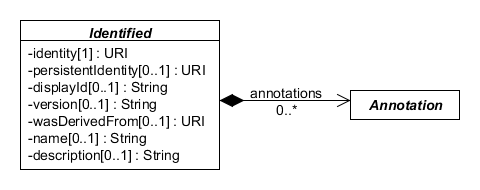
\includegraphics[scale=0.6]{uml/identified}
\caption[]{Diagram of the \sbol{Identified} abstract class and its associated properties}
\label{uml:identified}
\end{center}
\end{figure}
  
\subparagraph{The \sbolheading{displayId} property}
\label{sec:displayId}
The \sbol{displayId} property is an OPTIONAL identifier with a data type of \sbol{String}. This property is intended to be an intermediate between a URI and the \sbol{name} property that is machine-readable, but more human-readable than the full URI of an object.

If the \sbol{displayId} property is used, then its \sbol{String} value MUST be composed of only alphanumeric or underscore characters and MUST NOT begin with a digit.

\subparagraph{The \sbolheading{name} property}
\label{sec:name}

The \sbol{name} property is OPTIONAL and has a data type of \sbol{String}. This property is intended to be displayed to a human when visualizing an \sbol{Identified} object.

If an \sbol{Identified} object lacks a name, then software tools SHOULD instead display the object's \sbol{displayId} or URI.
It is RECOMMENDED that software tools give users the ability to switch perspectives between \sbol{name} properties that are human-readable and \sbol{displayId} properties that are less human-readable, but are more likely to be unique.

\subparagraph{The \sbolheading{description} property}
\label{sec:description}

The \sbol{description} property is OPTIONAL and has a data type of \sbol{String}. This property is intended to contain a more thorough text description of an \sbol{Identified} object.

\subparagraph{The \sbolheading{prov:wasDerivedFrom} property}
\label{sec:prov:wasDerivedFrom}
An \sbol{Identified} object can have zero or more \sbol{prov:wasDerivedFrom} properties, each of type URI. This property is defined by the PROV-O ontology and is located in the \url{https://www.w3.org/TR/prov-o/} namespace (Reference: \ref{sec:provenance}).

 An SBOL object with this property refers to one or more SBOL objects or non-SBOL resources from which this object was derived. An SBOL object MUST NOT refer to itself via its own \sbol{prov:wasDerivedFrom} property or form a cyclical chain of references via its \sbol{prov:wasDerivedFrom} property and those of other SBOL objects. For example, the reference chain ``$A$ was derived from $B$ and $B$ was derived from $A$'' is cyclical.

\subparagraph{The \sbolheading{prov:wasGeneratedBy} property}
\label{sec:prov:wasGeneratedBy}
An \sbol{Identified} object can have zero or more \sbol{prov:wasGeneratedBy} properties, each of type URI. This property is defined by the PROV-O ontology and is located in the \url{https://www.w3.org/TR/prov-o/} namespace (Reference: \ref{sec:provenance}).

An SBOL object with this property refers to one or more \sbol{prov:Activity} objects that describe how this object was generated.
Provenance history formed by \sbol{prov:wasGeneratedBy} properties of \sbol{Identified} objects and entity references in \sbol{prov:Usage} objects MUST NOT form circular reference chains.


\subsection {TopLevel}
\label{sec:TopLevel}
\sbol{TopLevel} is an abstract class that is extended by any \sbol{Identified} class that can be found at the top level of an SBOL document or file. In other words, \sbol{TopLevel} objects are not nested inside any other object via a composite aggregation or black diamond arrow association property. Instead of nesting, composite \sbol{TopLevel} objects refer to subordinate \sbol{TopLevel} objects by their \sbol{URI}s using shared aggregation or white diamond arrow association properties. The \sbol{TopLevel} classes defined in this specification are \sbol{Sequence}, \sbol{Component}, \sbol{Model}, \sbol{Collection}, \sbol{GenericTopLevel}, \sbol{CombinatorialDerivation}, and \sbol{Implementation}(\ref{uml:toplevel}).


\begin{figure}[ht]
\begin{center}
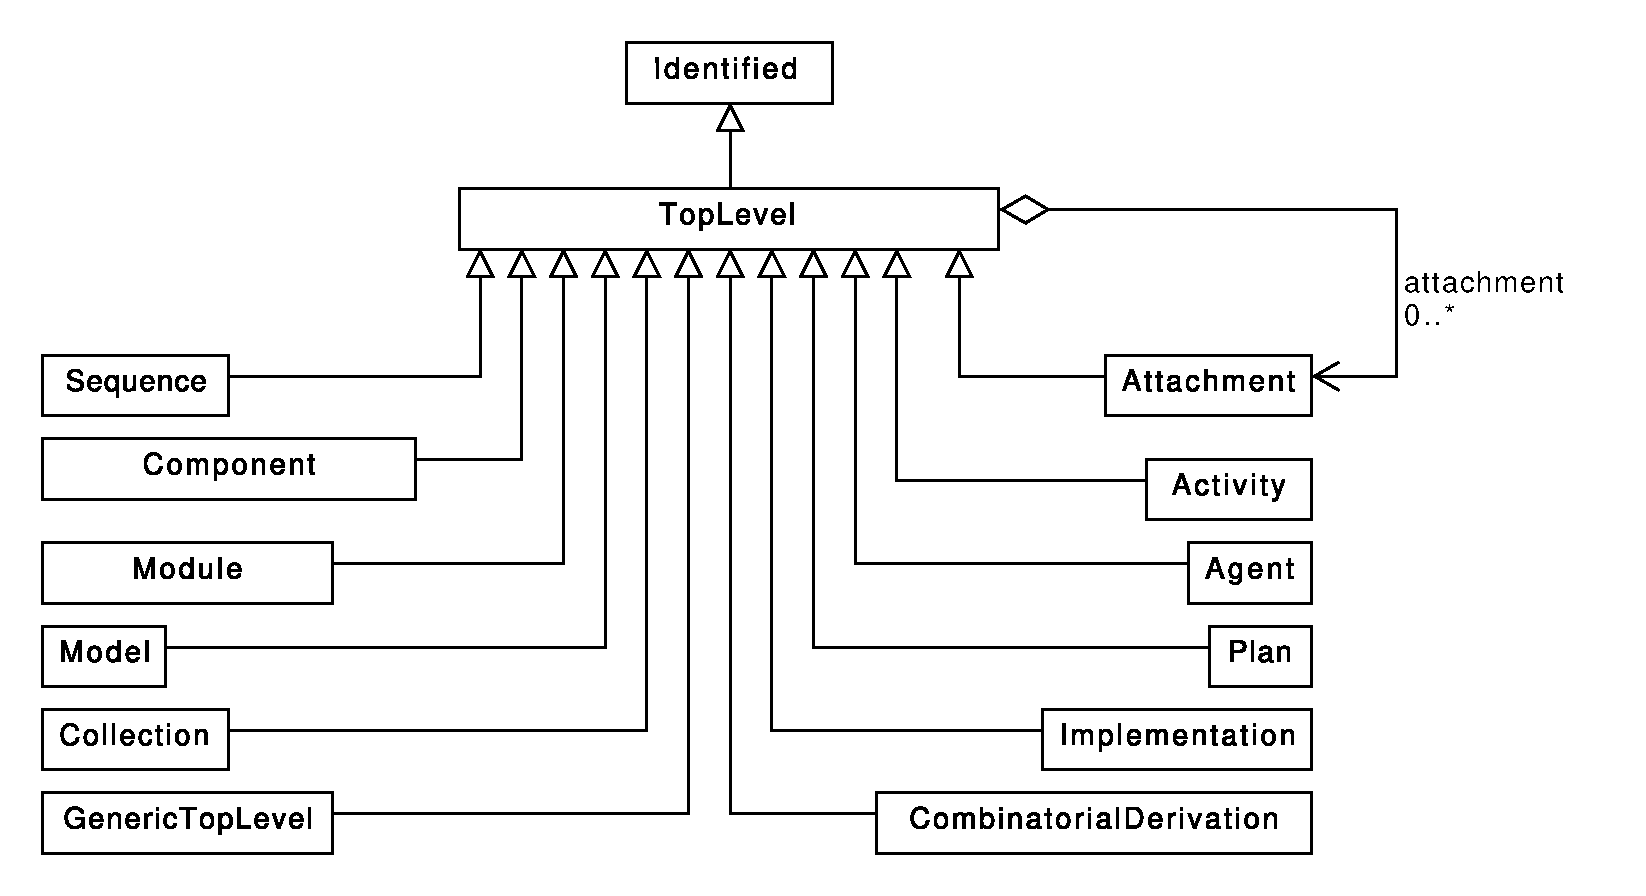
\includegraphics[width=\textwidth]{uml/toplevel}
\caption[]{Classes that inherit from the \sbol{TopLevel} abstract class.}
\label{uml:toplevel}
\end{center}
\end{figure}


\subparagraph{The hasAttachment property}
\label{sec:hasAttachment}
A \sbol{TopLevel} object can have zero or more \sbol{hasAttachment} properties, each of type URI specifying an \sbol{Attachment} object. The \sbol{Attachment} class is described in more detail in Section~\ref{sec:Attachment}.

\subsection{Sequence}
\label{sec:Sequence}
The purpose of the \sbol{Sequence} class is to represent the primary structure of a \sbol{Component} object and the manner in which it is encoded. This representation is accomplished  by means of the \sbol{elements} property and \sbol{encoding} property (\ref{uml:sequence}).

\begin{figure}[ht]
\begin{center}
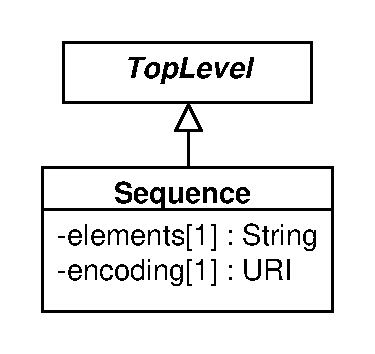
\includegraphics[scale=0.6]{uml/sequence}
\caption[]{Diagram of the \sbol{Sequence} class and its associated properties.}
\label{uml:sequence}
\end{center}
\end{figure}


\subparagraph{The \sbolheading{elements} property}
\label{sec:elements}
The \sbol{elements} property is a REQUIRED \sbol{String} of characters that represents the constituents of a biological or chemical molecule. For example, these characters could represent the nucleotide bases of a molecule of DNA, the amino acid residues of a protein, or the atoms and chemical bonds of a small molecule.

\subparagraph{The \sbolheading{encoding} property}
\label{sec:encoding}
The \sbol{encoding} property is REQUIRED and has a data type of \sbol{URI}. This property MUST indicate how the \sbol{elements} property of a \sbol{Sequence} MUST be formed and interpreted.

For example, the \sbol{elements} property of a \sbol{Sequence} with an \external{IUPAC DNA} encoding property MUST contain characters that represent nucleotide bases, such as {\tt a}, {\tt t}, {\tt c}, and {\tt g}. The \sbol{elements} property of a \sbol{Sequence} with a \external{Simplified Molecular-Input Line-Entry System (SMILES)} encoding, on the other hand, MUST contain characters that represent atoms and chemical bonds, such as {\tt C}, {\tt N}, {\tt O}, and {\tt =}.

\ref{tbl:sequence_encodings} provides a list of possible \sbol{URI} values for the \sbol{encoding} property. The terms in \ref{tbl:sequence_encodings} are organized by the type of \sbol{Component} (see \ref{tbl:component_types}) that typically refer to a \sbol{Sequence} with such an \sbol{encoding}. It is RECOMMENDED that the encoding property of a Sequence contains a URI from \ref{tbl:sequence_encodings}. When the \sbol{encoding} of a \sbol{Sequence} is well described by one of the \sbol{URI}s in \ref{tbl:sequence_encodings}, it MUST contain that \sbol{URI}.

More information on IUPAC encoding can be found at \url{http://www.bioinformatics.org/sms2/iupac.html}.

%A Summary of letters for nucleic acids and aminoacids
\begin{table}[ht]
  \begin{edtable}{tabular}{lll}
    \toprule
     \textbf{Encoding} & \textbf{URI} & \textbf{Component Type} \\
    \midrule
     IUPAC DNA, RNA & \url{http://www.chem.qmul.ac.uk/iubmb/misc/naseq.html} & DNA, RNA \\
    IUPAC Protein & \url{http://www.chem.qmul.ac.uk/iupac/AminoAcid/} & Protein\\
   SMILES & \url{http://www.opensmiles.org/opensmiles.html} & SmallMolecule \\
    \bottomrule
  \end{edtable}
  \caption{\sbol{URI}s for specifying the \sbol{encoding} property of a \sbol{Sequence}, organized by the type of \sbol{Component} (see \ref{tbl:component_types}) that typically refer to a \sbol{Sequence} with such an \sbol{encoding}.}
  \label{tbl:sequence_encodings}
\end{table}

\subsection{Component}
\label{sec:Component}

The \sbol{Component} class represents the structural and/or functional entities of a biological design. The primary usage of this class is to represent entities with designed sequences, such as DNA, RNA, and proteins, but it can also be used to represent any other entity that is part of a design, such as small molecules, molecular complexes, strains, samples, light, and abstract functional groupings of other entities.

As shown in \ref{uml:component}, the \sbol{Component} class describes a design entity using the following properties: \sbolmult{types:CD}{types}, \sbolmult{roles:CD}{roles}, \sbol{sequences}, \sbol{interactions}, and \sbol{models}. 
In addition, this class has properties for describing and organizing the substructure of said design entity, including \sbol{feature} and \sbol{constraint}.

\begin{figure}[ht]
\begin{center}
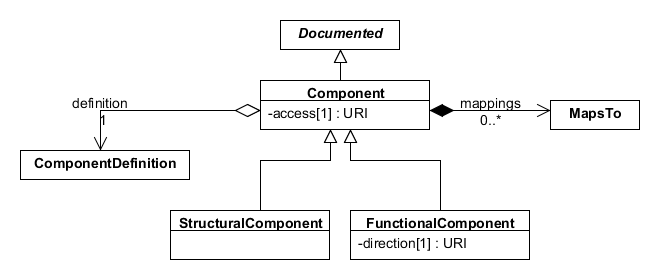
\includegraphics[width=0.95\textwidth]{uml/component}
\caption[]{Diagram of the \sbol{Component} class and its associated properties.}
\label{uml:component}
\end{center}
\end{figure} \todo{change diagram to reflect changes from SEP 41}

\subparagraph{The \sbolheading{types} property}
\label{sec:types:CD}

The \sbolmult{types:CD}{types} property is a REQUIRED set of \sbol{URI}s that
specifies the category of biochemical or physical entity (for example DNA,
protein, or small molecule) that a \sbol{Component} object abstracts
for the purpose of engineering design. For DNA or RNA entities,
additional \sbolmult{types:CD}{types} fields are used to describe nucleic acid
topology (circular / linear) and strandedness (double- or single-stranded).

The \sbolmult{types:CD}{types} property of every \sbol{Component} MUST contain one or more \sbol{URI}s that MUST identify terms from appropriate ontologies, such as the Systems Biology Ontology ~\cite{SBO} or  the ontology of Chemical Entities of Biological Interest (ChEBI) ~\cite{chebi}.
\ref{tbl:component_types} provides a list of possible ontology terms for the \sbolmult{types:CD}{types} property and their \sbol{URI}s.
In order to maximize the compatibility of designs, the \sbolmult{types:CD}{types} property of a \sbol{Component} SHOULD contain a \sbol{URI} from \ref{tbl:component_types}, and any \sbol{Component} that can be well-described by one of the terms in \ref{tbl:component_types} MUST use the \sbol{URI} for that term as one of its \sbolmult{types:CD}{types}.
Finally, if the \sbolmult{types:CD}{types} property contains multiple \sbol{URI}s, then they MUST identify non-conflicting terms (otherwise, it might not be clear how to interpret them). For example, the SBO terms provided by \ref{tbl:component_types} would conflict because they specify classes of biochemical entities with different molecular structures.

\begin{table}[ht]
  \begin{edtable}{tabular}{ll}
    \toprule
    \textbf{Component Type} & \textbf{URI for SBO Term} \\
    \midrule
    DNA (Deoxyribonucleic acid)  & \url{https://identifiers.org/SBO:0000251}\\
    RNA (Ribonucleic acid) & \url{https://identifiers.org/SBO:0000251}\\
    Protein (Polypeptide chain)  & \url{https://identifiers.org/SBO:0000252}\\
    Simple Chemical  & \url{https://identifiers.org/SBO:0000247}\\
    Non-covalent complex  & \url{https://identifiers.org/SBO:0000253}\\
    \bottomrule
  \end{edtable}
  \caption{SBO terms to specify the molecule type using the \sbolmult{types:CD}{types} property of a \sbol{Component}.}
 \label{tbl:component_types}
\end{table}

\emph{Nucleic Acid Topology types}\\
\vspace{-7pt}

Any \sbol{Component} classified as DNA (see \ref{tbl:component_types}) is RECOMMENDED to encode circular/linear topology information in an additional type field. This
(topology) type field SHOULD specify a URI from the Topology Attribute branch of the SO
(this is currently just 'linear' or 'circular' as given in \ref{tbl:component_topology}). Topology information SHOULD be specified for DNA \sbol{Component} records with a fully specified sequence, except in three scenarios: if the DNA record doesn't have sequence information, or if the DNA record has incomplete sequence information, or if topology is genuinely unknown. For any \sbol{Component} classified as RNA (see \ref{tbl:component_types}), a topology type field is OPTIONAL. The default
assumption in this case is linear topology.  In any case, no more than one topology should be specified.

Any \sbol{Component} classified as DNA or RNA MAY also have strand
information encoded in an additional (third) type field using a URI from the Strand Attribute branch of the SO (currently there are only two possible terms for single or double-stranded nucleic
acids given in \ref{tbl:component_topology}). In absence of this field, the
default strand information assumed for DNA is 'double-stranded' and for RNA is
'single-stranded'. 

Any other type of \sbol{Component} record (protein, small molecule, etc) SHOULD NOT
have any type field pointing to SO terms from the topology or strand attribute branches of SO.

Note that a \emph{circular} topology instructs software to interpret the
beginning / end position of a given sequence (be it DNA or RNA) as arbitrary so
that sequence features may be mapped or identified across this junction. \emph{Double stranded} instructs software to apply sequence searches to both strands (i.e. sequence and reverse complement of sequence).

\begin{table}[ht]
  \begin{edtable}{tabular}{ll}
    \toprule
    \textbf{Nucleic Acid Topology} & \textbf{URI for Nucleic Acid Topology
      Term in SO} \\
    \midrule
    linear  & \url{http://identifiers.org/so/SO:0000987}\\
    circular  & \url{http://identifiers.org/so/SO:0000988}\\
    single-stranded & \url{http://identifiers.org/so/SO:0000984}\\
    double-stranded & \url{http://identifiers.org/so/SO:0000985}\\
    \bottomrule
  \end{edtable}
  \caption{Sequence Ontology terms to encode DNA or RNA topology information in the \sbolmult{types:CD}{types} properties of a \sbol{Component}.}
 \label{tbl:component_topology}
\end{table}

\subparagraph{The \sbolheading{roles} property}
\label{sec:roles:CD}

The \sbolmult{roles:CD}{roles} property is an OPTIONAL set of \sbol{URI}s that clarifies the potential function of the entity represented by a \sbol{Component} in a biochemical or physical context.

The \sbolmult{roles:CD}{roles} property of a \sbol{Component} MAY contain one or more \sbol{URI}s that MUST identify terms from ontologies that are consistent with the \sbolmult{types:CD}{types} property of the \sbol{Component}.
For example, the \sbolmult{roles:CD}{roles} property of a DNA or RNA \sbol{Component} could contain URIs identifying terms from the Sequence Ontology (SO). As a best practice, a DNA or RNA \sbol{Component} SHOULD contain exactly one \sbol{URI} that refers to a term from the sequence feature branch of the SO.
Similarly, the roles property of a Protein and SmallMolecule \sbol{Component} SHOULD respectively contain \sbol{URI}s identifying terms from the \texttt{MolecularFunction} branch (\texttt{GO:0003674}) of the Gene Ontology (GO) and the \texttt{role} branch (\texttt{CHEBI:50906}) of the CHEBI ontology.
\ref{tbl:component_roles} contains a list of possible ontology terms for the \sbolmult{roles:CD}{roles} property and their \sbol{URI}s. These terms are organized by the type of \sbol{Component} to which they SHOULD apply (see \ref{tbl:component_types}). Any \sbol{Component} that can be well-described by one of the terms in \ref{tbl:component_roles} MUST use the \sbol{URI} for that term as one of its \sbolmult{roles:CD}{roles}.

These \sbol{URI}s might identify descriptive biological roles, such as ``metabolic pathway'' and ``signaling cascade,'' but they can also identify identify ``logical'' roles, such as ``inverter'' or ``AND gate'', or other abstract roles for describing the function of design. Interpretation of the meaning of such roles currently depends on the software tools that read and write them.


\begin{table}[ht]
  \begin{edtable}{tabular}{lll}
    \toprule
    \textbf{Component Role} & \textbf{URI for Ontology Term} & \textbf{Component Type} \\
    \midrule
   Promoter & \url{http://identifiers.org/so/SO:0000167} & DNA \\
   RBS & \url{http://identifiers.org/so/SO:0000139} & DNA \\
      CDS & \url{http://identifiers.org/so/SO:0000316} & DNA \\
      Terminator & \url{http://identifiers.org/so/SO:0000141} & DNA \\
      Gene & \url{http://identifiers.org/so/SO:0000704} & DNA \\
      Operator & \url{http://identifiers.org/so/SO:0000057} & DNA \\
      Engineered Gene & \url{http://identifiers.org/so/SO:0000280} & DNA \\
      mRNA & \url{http://identifiers.org/so/SO:0000234} & RNA \\
      Effector & \url{http://identifiers.org/chebi/CHEBI:35224} & Small Molecule \\
      Transcription Factor & \url{http://identifiers.org/go/GO:0003700} & Protein\\
    \bottomrule
  \end{edtable}
  \caption{Ontology terms to specify the \sbolmult{roles:CD}{roles} property of a \sbol{Component}, organized by the type of \sbol{Component} to which they are intended to apply (see \ref{tbl:component_types}).}
  \label{tbl:component_roles}
\end{table}


\subparagraph{The \sbolheading{feature} property}
\label{sec:feature}

The \sbol{feature} property MAY have one or more \sbol{Feature} properties. The set of relations between \sbol{Feature} and \sbol{Component} objects is strictly acyclic (see \ref{sec:Feature}).

While the \sbol{Component} class is analogous to a blueprint or specification sheet for a biological part, the \sbol{Feature} class represents the specific occurrence of a part within a design.
Hence, this class allows a biological design to include multiple instances of a particular part (defined by reference to the same \sbol{Component}). For example, the \sbol{Component} of a polycistronic gene could contain two \sbol{Feature} objects that refer to the same \sbol{Component} of a CDS.

The \sbol{feature} properties of \sbol{Component} objects can be used to construct a hierarchy of \sbol{Feature} and \sbol{Component} objects.
If a \sbol{Component} in such a hierarchy refers to a \sbol{Location} object, and there exist a \sbol{Component} objects lower in the hierarchy that refer to \sbol{Location} object that referes to the same \sbol{Sequence} with the same \sbol{encoding}, then the \sbol{elements} properties of these \sbol{Sequence} objects SHOULD be consistent with each other, such that well-defined mappings exist from the ``lower level'' \sbol{elements} to the ``higher level'' \sbol{elements} in accordance with their shared \sbol{encoding} properties. This mapping is also subject to any restrictions on the positions of the \sbol{Feature} objects in the hierarchy that are imposed by the \sbol{SequenceFeature} or \sbol{SequenceConstraint} objects contained by the \sbol{Component} objects in the hierarchy.

A DNA \sbol{Component}, for example, could refer to a \sbol{Sequence} with an \external{IUPAC DNA} \sbol{encoding} and an \sbol{elements} \external{String} of ``{\tt gattaca}.'' In turn, this \sbol{Component} could contain a \sbol{Feature} that refers to a ``lower level''  \sbol{Component} that also refers to a \sbol{Sequence} with an \external{IUPAC DNA} \sbol{encoding}. Consequently, a consistent \sbol{elements} \external{String} of this ``lower level'' \sbol{Sequence} could be ``{\tt gatta},'' or perhaps ``{\tt tgta}'' if the \sbol{Feature} is positioned by a \sbol{SequenceAnnotation} that contains a \sbol{Location}  with an \sbol{orientation} of ``reverse complement'' (see \ref{sec:Location}).

While the \sbol{Component} class is analogous to a specification sheet for a system of interacting biological elements, the \sbol{Feature} class represents the occurrence of a particular subsystem within the system.
Hence, this class allows a system design to include multiple instances of a subsystem, all defined by reference to the same \sbol{Component}.
For example, consider the \sbol{Component} for a network of two-input repressor devices in which the particular repressors have not been chosen yet. This \sbol{Component} could contain multiple \sbol{Feature} objects that refer to the same \sbol{Component} of an abstract two-input repressor device.

Just as a \sbol{Feature} represents an instance of a subsystem in the overall system represented by a  \sbol{Component}, a \sbol{Feature} represents an instance of a structural entity (represented by a \sbol{Component}) in the system. This concept allows a \sbol{Component} to assert different interactions for separate copies of the same structural entity if needed. For example, a \sbol{Component} might contain multiple \sbol{Feature}  objects that refer to the same promoter \sbol{Component}, but assert different interactions for these promoter copies based on their separate positions in another \sbol{Component} that represents the structure of the entire system.

\todo{Do not delete commented out section. we may need part of it later.}
%In addition, each \sbol{SubComponent} can  position a \sbol{Feature} of the \sbol{Component} at the region specified by its \sbol{Location} objects (see \ref{sec:Location}).
%The \sbol{feature} property MUST NOT contain two or more \sbol{SequenceFeature} objects that refer to the same \sbol{Feature} in this way.

%Finally, as a best practice, if a \sbol{Component} refers to a \sbol{Sequence} with an \external{IUPAC} \sbol{encoding} from \ref{tbl:sequence_encodings}, then each of its \sbol{SequenceFeature} objects that contains a \sbol{Range} or \sbol{Cut} SHOULD specify a region on the \sbol{elements} of this \sbol{Sequence}.
%For example, the \sbol{Component} of a eukaryotic gene could refer to a \sbol{Sequence} with an \external{IUPAC DNA} \sbol{encoding}. In order to specify the discontiguous region occupied by its CDS, this gene \sbol{Component} would need a \sbol{SequenceFeature} that contains one or more \sbol{Range} objects, each one specifying \sbol{start} and \sbol{end} positions that correspond to indices of the \sbol{elements} of its DNA \sbol{Sequence}.

\subparagraph{The \sbolheading{constraint} property}
\label{sec:constraint}

The \sbol{constraint} property is OPTIONAL and MAY contain a set of \sbol{Constraint} objects. 
These objects describe any restrictions on the relative, sequence-based positions and/or orientations of the \sbol{Feature} objects contained by the \sbol{Component}.
For example, the \sbol{Component} of a gene might specify that the position of its promoter \sbol{Feature} precedes that of its CDS \sbol{Feature}. This is particularly useful when a \sbol{Component} lacks a \sbol{Sequence} and therefore cannot specify the precise, sequence-based positions of its \sbol{Feature} objects using \sbol{SubComponent} objects using \sbol{Location} objects.

\subparagraph{The \sbolheading{interactions} property}\label{sec:interactions}

The \sbol{interactions} property is OPTIONAL and MAY specify a set of \sbol{Interaction} objects within the \sbol{Component}.

The \sbol{Interaction} class provides an abstract, machine-readable representation of entity behavior within a \sbol{Component} (whereas a more detailed model of the system might not be suited to machine reasoning, depending on its implementation).
Each \sbol{Interaction} contains \sbol{Participation} objects that indicate the roles of the \sbol{Feature} objects involved in the \sbol{Interaction}.

\subparagraph{The \sbolheading{models} property}\label{sec:models}
The \sbol{models} property is OPTIONAL and MAY specify a set of \sbol{URI} references to \sbol{Model} objects.

\sbol{Model} objects are placeholders that link \sbol{Component} objects to computational models of any format.
A \sbol{Component} object can link to more than one \sbol{Model} since each might encode system behavior in a different way or at a different level of detail.

\subsubsection{Interaction}
\label{sec:Interaction}

\begin{figure}[ht]
\begin{center}
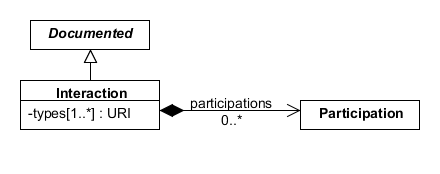
\includegraphics[scale=0.6]{uml/interaction}
\caption[]{Diagram of the \sbol{Interaction} class and its associated properties.}
\label{uml:interaction}
\end{center}
\end{figure}

The \sbol{Interaction} class provides more detailed description of how the \sbol{Feature} objects of a\\ \sbol{Component} are intended to work together.
For example, this class can be used to represent different forms of genetic regulation (e.g., transcriptional activation or repression), processes from the central dogma of biology (e.g. transcription and translation), and other basic molecular interactions (e.g., non-covalent binding or enzymatic phosphorylation).
Each \sbol{Interaction} includes a \sbolmult{types:I}{types} property that refers to descriptive ontology terms and a \sbol{participations} property that describes which \sbol{Feature} objects participate in the \sbol{Interaction}.

\subparagraph{The \sbolheading{types} property}\label{sec:types:I}

The \sbolmult{types:I}{types} property is a REQUIRED set of \sbol{URI}s that describes the behavior represented by an \sbol{Interaction}.

The \sbolmult{types:I}{types} property MUST contain one or more \sbol{URI}s that MUST identify terms from appropriate ontologies. It is RECOMMENDED that exactly one \sbol{URI} contained by the \sbolmult{types:I}{types} property refer to a term from the occurring entity branch of the Systems Biology Ontology (SBO). (See \url{http://www.ebi.ac.uk/sbo/main/}) \ref{tbl:interaction_types} provides a list of possible SBO terms for the \sbolmult{types:I}{types} property and their corresponding \sbol{URI}s.

\begin{table}[ht]
  \begin{edtable}{tabular}{ll}
    \toprule
    \textbf{Interaction Type} & \textbf{URI for SBO Term} \\
    \midrule
    Inhibition  & \url{http://identifiers.org/biomodels.sbo/SBO:0000169}\\
    Stimulation & \url{http://identifiers.org/biomodels.sbo/SBO:0000170}\\
    Biochemical Reaction & \url{http://identifiers.org/biomodels.sbo/SBO:0000176}\\
    Non-Covalent Binding & \url{http://identifiers.org/biomodels.sbo/SBO:0000177}\\
    Degradation & \url{http://identifiers.org/biomodels.sbo/SBO:0000179}\\
    Genetic Production & \url{http://identifiers.org/biomodels.sbo/SBO:0000589}\\
    Control  & \url{http://identifiers.org/biomodels.sbo/SBO:0000168} \\
    \bottomrule
  \end{edtable}
  \caption{SBO terms to specify the \sbolmult{types:I}{types} property of an \sbol{Interaction}.}
  \label{tbl:interaction_types}
\end{table}

If an \sbol{Interaction} is well described by one of the terms from \ref{tbl:interaction_types}, then its \sbolmult{types:I}{types} property MUST contain the \sbol{URI} that identifies this term. Lastly, if the \sbolmult{types:I}{types} property of an \sbol{Interaction} contains multiple
 \sbol{URI}s, then they MUST identify non-conflicting terms. For example, the SBO terms ``stimulation'' and ``inhibition'' would conflict.

\subparagraph{The \sbolheading{participations} property}\label{sec:participations}

The \sbol{participations} property is an OPTIONAL and MAY contain a set of \sbol{Participation} objects, each of which identifies the \sbolmult{roles:P}{roles} that its referenced \sbol{Feature} plays in the \sbol{Interaction}.

Even though an \sbol{Interaction} generally contains at least one \sbol{Participation}, the case of zero \sbol{Participation} objects is allowed because it is plausible that a designer might want to specify that an \sbol{Interaction} will exist, even if its \sbol{participant}s have not yet been determined.

\begin{figure}[ht]
\begin{center}
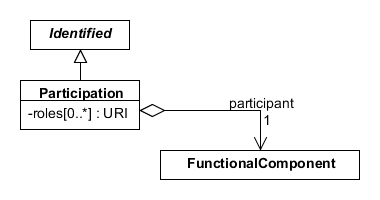
\includegraphics[scale=0.6]{uml/participation}
\caption[]{Diagram of the \sbol{Participation} class and its associated properties.}
\label{uml:participation}
\end{center}
\end{figure}

\subsubsection{Participation}
\label{sec:Participation}

Each \sbol{Participation} represents how a particular \sbol{Feature} behaves in its parent
\sbol{Interaction}.

\subparagraph{The \sbolheading{roles} property}\label{sec:roles:P}

The \sbolmult{roles:P}{roles} property is a REQUIRED set of \sbol{URI}s that describes the behavior of a \sbol{Participation} (and by extension its referenced \sbol{Feature}) in the context of its parent \sbol{Interaction}.

The \sbolmult{roles:P}{roles} property MUST contain one or more \sbol{URI}s that MUST identify terms from appropriate ontologies. It is RECOMMENDED that exactly one \sbol{URI} contained by the \sbolmult{roles:P}{roles} property refer to a term from the participant role branch of the SBO. \ref{tbl:participant_roles} provides a list of possible SBO terms for the \sbolmult{roles:P}{roles} property and their corresponding \sbol{URI}s.

\begin{table}[ht]
  \begin{edtable}{tabular}{lll}
    \toprule
    \textbf{Participation Role} & \textbf{URI for SBO Term} & \textbf{Interaction Types}\\
    \midrule
    Inhibitor  & \url{http://identifiers.org/biomodels.sbo/SBO:0000020} & Inhibition\\
    Inhibited  & \url{http://identifiers.org/biomodels.sbo/SBO:0000642} & Inhibition\\
    Stimulator & \url{http://identifiers.org/biomodels.sbo/SBO:0000459}  & Stimulation\\
    Stimulated & \url{http://identifiers.org/biomodels.sbo/SBO:0000643}  & Stimulation\\
     Reactant & \url{http://identifiers.org/biomodels.sbo/SBO:0000010}  & Non-Covalent Binding, Degradation \\
     & & Biochemical Reaction \\
    Product & \url{http://identifiers.org/biomodels.sbo/SBO:0000011}  & Non-Covalent Binding, \\
    & & Genetic Production, Biochemical Reaction\\
    Promoter  & \url{http://identifiers.org/biomodels.sbo/SBO:0000598} & Inhibition, Stimulation, Genetic Production\\
    Modifier  & \url{http://identifiers.org/biomodels.sbo/SBO:0000019} & Biochemical Reaction, Control\\
    Modified  & \url{http://identifiers.org/biomodels.sbo/SBO:0000644} & Biochemical Reaction, Control\\
    Template  & \url{http://identifiers.org/biomodels.sbo/SBO:0000645} & Genetic Production\\
%    Ligand & \url{http://identifiers.org/biomodels.sbo/SBO:0000280}\\
%    Non-Covalent Complex & \url{http://identifiers.org/biomodels.sbo/SBO:0000253}\\
    \bottomrule
  \end{edtable}
  \caption{SBO terms to specify the \sbolmult{roles:P}{roles} property of a \sbol{Participation}.}
  \label{tbl:participant_roles}
\end{table}

If a \sbol{Participation} is well described by one of the terms from \ref{tbl:participant_roles}, then its \sbolmult{roles:P}{roles} property MUST contain the \sbol{URI} that identifies this term.
Also, if a \sbol{Participation} belongs to an \sbol{Interaction} that has a type listed in \ref{tbl:interaction_types}, then the \sbol{Participation} SHOULD have a role that is cross-listed with this type in \ref{tbl:participant_roles}.
Lastly, if the \sbolmult{roles:P}{roles} property of a \sbol{Participation} contains multiple
 \sbol{URI}s, then they MUST identify non-conflicting terms. For example, the SBO terms ``stimulator'' and ``inhibitor'' would conflict.


\subparagraph{The \sbolheading{participant} property}\label{sec:participant}

The \sbol{participant} property MUST specify precisely one \sbol{Feature} object that plays the designated role in its parent \sbol{Interaction} object.


\subsubsection{Interface}
\label{sec:Interface}

\begin{figure}[ht]
\begin{center}
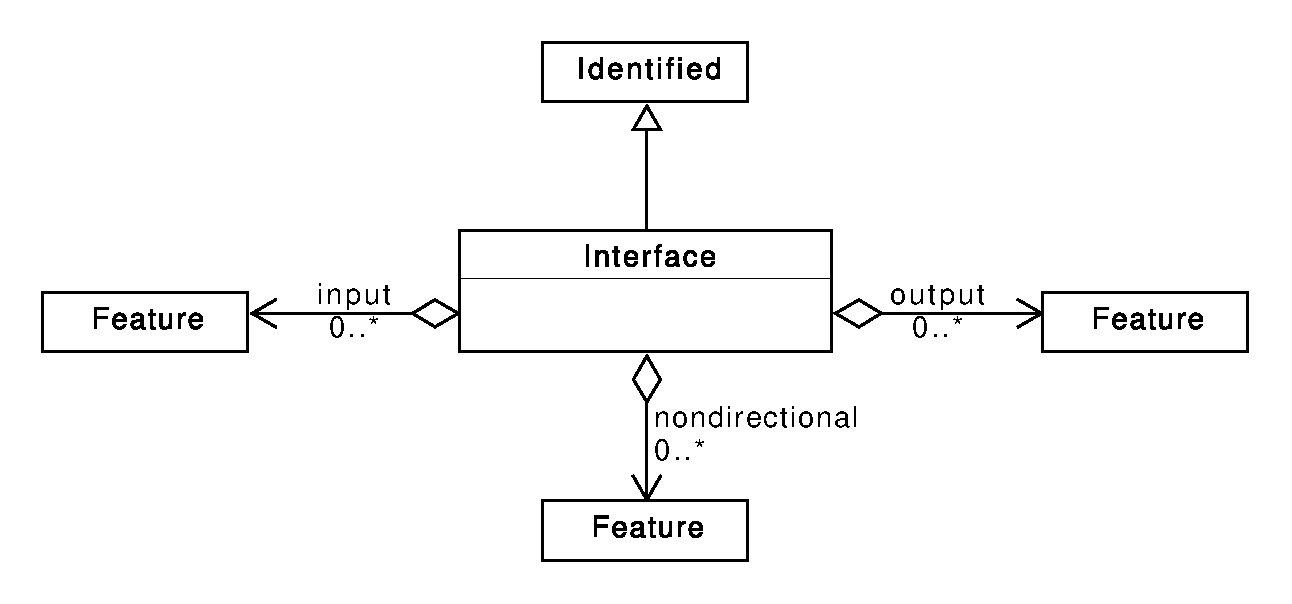
\includegraphics[scale=0.6]{uml/interface}
\caption[]{Diagram of the \sbol{Interface} class and its associated properties.}
\label{uml:interface}
\end{center}
\end{figure}

The \sbol{Interface} class is a way of explicitly specifying the interface of a \sbol{Component}. 

\subparagraph{The \sbolheading{input} property}
\label{sec:input:Interface}
The \sbolmult{input:Interface}{input} property is OPTIONAL and MAY contain a set of \sbol{Feature} \sbol{URI}s in the same \sbol{Component}.
\subparagraph{The \sbolheading{output} property}
\label{sec:output:Interface}
The \sbolmult{output:Interface}{output} property is OPTIONAL and MAY contain a set of \sbol{Feature} \sbol{URI}s in the same \sbol{Component}.

\subparagraph{The \sbolheading{nondirectional} property}
\label{sec:nondirectional:Interface}
The \sbolmult{nondirectional:Interface}{nondirectional} property is OPTIONAL and MAY contain a set of \sbol{Feature} \sbol{URI}s in the same \sbol{Component}. Note that nondirectional can imply both bidirectional as well as situations where there are no flows (for instance - a physical interface).


\subsubsection{Feature}
\label{sec:Feature}

\begin{figure}[ht]
\begin{center}
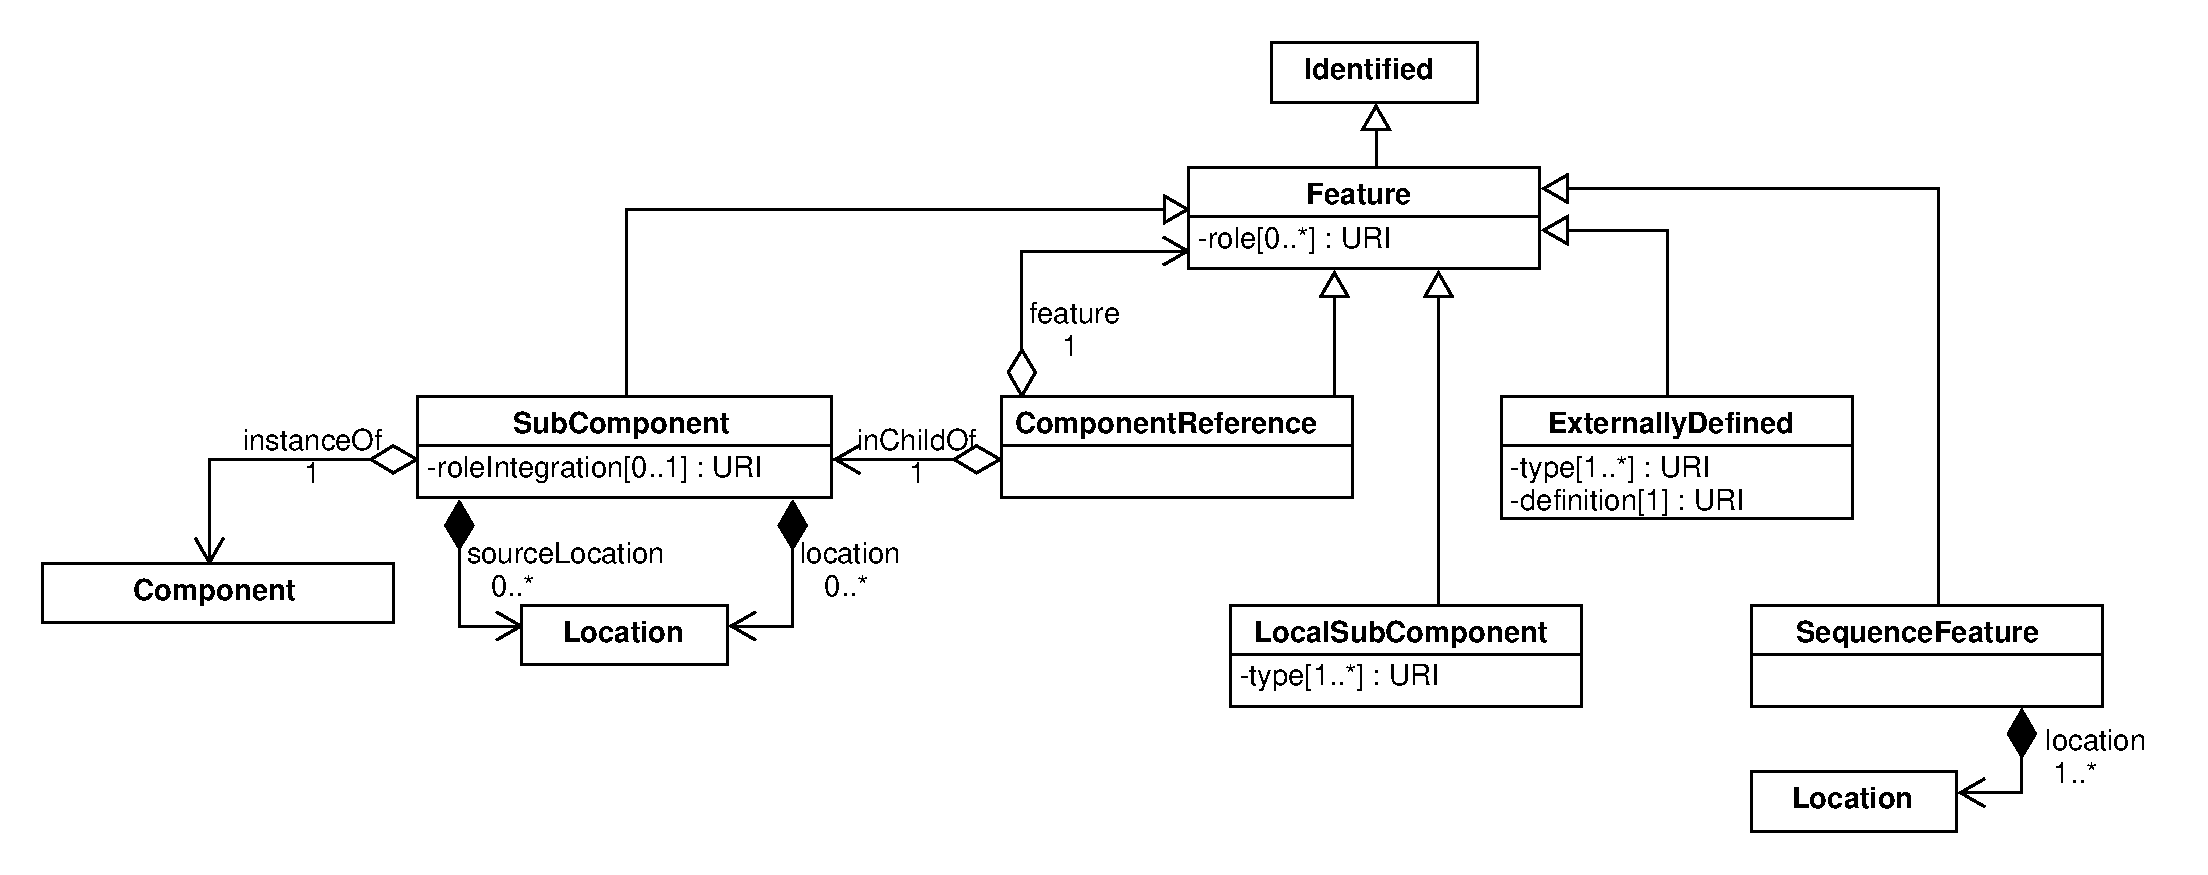
\includegraphics[width=\textwidth]{uml/feature}
\caption[]{Diagram of the \sbol{Feature} class and its associated properties.}
\label{uml:subcomponent}
\end{center}
\end{figure}

The \sbol{Feature} class is used to compose \sbol{Component} objects into a structural or functional hierarchy. 

\subparagraph{The \sbolheading{role} property}\label{sec:roles:C}

The expected purpose and function of a genetic part are described by the
\sbolmult{roles:CD}{roles} property of \sbol{Component}. However, the same building block might be used for a different purpose in an actual design. In other words, purpose and function are sometimes determined by context. 

The \sbolmult{roles:C}{roles} property comprises an OPTIONAL set of zero or more \sbolmult{roles:C}{role} \sbol{URI}s describing the purpose or potential function of this \sbol{Feature}'s included sub-\sbol{Component} in the \textit{context} of its parent \sbol{Component}.
If provided, these \sbolmult{roles:C}{role} \sbol{URI}s MUST identify terms from appropriate ontologies. Roles are not restricted to describing biological function; they may annotate a \sbol{Feature}'s function in any domain for which an ontology exists.

It is RECOMMENDED that these \sbolmult{roles:C}{role} \sbol{URI}s identify terms that are compatible with the \sbolmult{types:CD}{type} properties of both this \sbol{Feature}'s parent \sbol{Component} and its included sub-\sbol{Component}. For example, a \sbolmult{roles:C}{role} of a \sbol{Feature} which belongs to a \sbol{Component} of type DNA and includes a sub-\sbol{Component} of type DNA might refer to terms from the Sequence Ontology. A table of recommended ontology terms for \sbolmult{roles:C}{roles} is given in \ref{tbl:component_roles}.

\paragraph{SubComponent}
\label{sec:SubComponent}

The \sbol{SubComponent} class a subclass of the \sbol{Feature} class that can be used to specify structural hierarchy. For example, the \sbol{Component} of a gene could contain four \sbol{SubComponent} objects: a promoter, RBS, CDS, and terminator. In turn, the \sbol{Component} of the promoter \sbol{SubComponent} could contain \sbol{SubComponent} objects defined as various operator sites.

\subparagraph{The \sbolheading{roleIntegration} property}\label{sec:roleIntegration:C}


A \sbolmult{roleIntegration:C}{roleIntegration} specifies the relationship between a \sbol{Feature} instance's own set of \sbolmult{roles:C}{roles} and the set of \sbolmult{roles:CD}{roles} on the included sub-\sbol{Component}.

The \sbolmult{roleIntegration:C}{roleIntegration} property has a data type of \sbol{URI}. A \sbol{Feature} instance with zero \sbolmult{roles:C}{roles} MAY OPTIONALLY specify a \sbolmult{roleIntegration:C}{roleIntegration}. A \sbol{Feature} instance with one or more \sbolmult{roles:C}{roles} MUST specify a \sbolmult{roleIntegration:C}{roleIntegration} from \ref{tbl:component_roleIntegration}.
If zero \sbol{Feature} \sbolmult{roles:C}{roles} are given and no \sbol{Feature} \sbolmult{roleIntegration:C}{roleIntegration} is given, then \url{http://sbols.org/v2\#mergeRoles} is assumed.
It is RECOMMENDED to specify a set of \sbol{Feature} \sbolmult{roles:C}{roles} only if the integrated result set of roles would differ from the set of \sbolmult{roles:CD}{roles} belonging to this \sbol{Feature}'s included sub-\sbol{Component}.


\begin{table}[ht]
  \begin{edtable}{tabular}{lp{4in}}
    \toprule
    \textbf{roleIntegration URI} & \textbf{Description} \\
    \midrule
    \url{http://sbols.org/v2\#overrideRoles} & In the context of this \sbol{Feature}, ignore any \sbolmult{roles:CD}{roles} given for the included sub-\sbol{Component}. Instead use only the set of zero or more \sbolmult{roles:C}{roles} given for this \sbol{Feature}. \\
    \url{http://sbols.org/v2\#mergeRoles} & Use the union of the two sets: both the set of zero or more \sbolmult{roles:C}{roles} given for this \sbol{Feature} as well as the set of zero or more \sbolmult{roles:CD}{roles} given for the included sub-\sbol{Component}. \\
    \bottomrule
  \end{edtable}
  \caption{Each \sbolmult{roleIntegration:C}{roleIntegration} mode is associated with a rule governing how a \sbol{Feature}'s roles are to be combined with the included 
sub-\sbol{Component}'s roles.}
  \label{tbl:component_roleIntegration}
\end{table}


\subparagraph{The \sbolheading{instanceOf} property}
\label{sec:instanceOf}

The \sbol{instanceOf} property is a REQUIRED \sbol{URI} that refers to the \sbol{Component} of the \sbol{Feature}.
As described in the previous section, this \sbol{Component} effectively provides information about the \sbolmult{types:CD}{types} and \sbolmult{roles:CD}{roles} of the \sbol{Feature}.

The \sbol{instanceOf} property MUST NOT refer to the same \sbol{Component} as the one that contains the \sbol{Feature}.
Furthermore, \sbol{Feature} objects MUST NOT form a cyclical chain of references via their \sbol{instanceOf} properties and the \sbol{Component} objects that contain them.
For example, consider the \sbol{Feature} objects $A$ and $B$ and the \sbol{Component} objects $X$ and $Y$. The reference chain ``$X$ contains $A$, $A$ is defined by $Y$, $Y$ contains $B$, and $B$ is defined by $X$'' is cyclical.

The \sbol{sourceLocations} property is an OPTIONAL set of zero or more \sbol{Location} objects that indicate which \sbol{elements} of a \sbol{Component}'s \sbol{Sequence} are to be included in the \sbol{Component}'s parent. The \sbol{sourceLocations} property
allows for only a portion of a \sbol{Component}'s \sbol{Sequence} to be included, rather than its entirety.

If the \sbol{sourceLocation} property is not set, then the whole \sbol{Sequence} is assumed to be included. Alternatively,
if the \sbol{sourceLocation} property is set, then the relationship between the original \sbol{Component}'s
\sbol{Sequence} and the included \sbol{Sequence} is defined identically to the \sbol{locations}
property on the \sbol{SequenceFeature} object.


\subparagraph{The \sbolheading{location} property}\label{sec:location}
The \sbol{location} property is an OPTIONAL set which points to a \sbol{Location} on the parent \sbol{Component} sequence; if \sbol{location} is missing, this indicates a part / sub-part relationship for which sequence details have not (yet) been determined.

The \sbol{Location} record(s) specified by a \sbol{Feature} are subject to the same restrictions currently in place for \sbol{SequenceFeature} \sbol{Location}. Concretely, two \sbol{Location} records attached to the same \sbol{Feature} MUST NOT overlap in their range as it would not be clear what that means. The \sbol{Location} of two separate \sbol{Feature}s may overlap.

\subparagraph{The \sbolheading{orientation} property}\label{sec:orientation2}
The \sbol{orientation} property is OPTIONAL and has a data type of \sbol{URI}. All subclasses of \sbol{Feature} share this property, which can be used to indicate how the region specified by the \sbol{SequenceFeature} and any associated double-stranded \sbol{SubComponent} is oriented on the \sbol{elements} of a \sbol{Sequence}  from their parent \sbol{Component}. \ref{tbl:orientation_types} provides a list of REQUIRED \sbol{orientation} \sbol{URI}s. If a \sbol{Feature} object has an \sbol{orientation}, then it MUST come from \ref{tbl:orientation_types}.

\todo{add best practice here talking about EntireComponent?}


\paragraph{ComponentReference}
\label{sec:ComponentReference}

The \sbol{ComponentReference} class is a subclass of \sbol{Feature} and a sibling of the \sbol{SubComponent} class. 


\subparagraph{The \sbolheading{inChildOf} property}\label{sec:inChildOf}

The \sbol{inChildOf} property is a REQUIRED \sbol{URI} that refers to a SubComponent. \sbol{inChildOf} must refer to a \sbol{SubComponent} pointed directly to by the parent of the \sbol{ComponentReference} (i.e., as a \sbol{SubComponent} of \sbol{Component}, or an \sbol{inChildOf} of \sbol{ComponentReference}). If the \sbol{Feature} is a \sbol{SubComponent}, then it must be a child of the \sbol{SubComponent} pointed to by \sbol{inChildOf}.

\subparagraph{The \sbolheading{feature} property}\label{sec:feature:CR}

The \sbolmult{feature:CR}{feature} property is an OPTIONAL \sbol{URI} that refers to a \sbol{Feature}.

\paragraph{LocalSubComponent}
\label{sec:LocalSubComponent}

The \sbol{LocalSubComponent} class a subclass of \sbol{Feature}. This class was serves as a way to create an ``empty'' \sbol{Component} to serve as a placeholder in more complex \sbol{Component}s. 

\subparagraph{The \sbolheading{type} property}\label{sec:type:LSC}

The \sbolmult{type:LSC}{type} property is REQUIRED and contains one or more \sbol{URI}s. The \sbolmult{type:ER}{type} property is identical to its use in \sbol{Component}

\paragraph{ExternallyDefined}
\label{sec:ExternallyDefined}

The \sbol{ExternallyDefined} class has been introduced so that external definitions in databases like CHEBI or UniProt can be referenced.

\subparagraph{The \sbolheading{type} property}\label{sec:type:ER}

The \sbolmult{type:ER}{type} property is REQUIRED and contains one or more \sbol{URI}s. The \sbolmult{type:ER}{type} property is identical to its use in \sbol{Component}

\subparagraph{The \sbolheading{definition} property}\label{sec:definition:ER}

The \sbolmult{definition:ER}{definition} property is REQUIRED and contains one \sbol{URI} that links to a cononical definition external to SBOL.


\paragraph{SequenceFeature}
\label{sec:SequenceFeature}

The \sbol{SequenceFeature} class describes one or more regions of interest on the \sbol{Sequence} objects referred to by its parent \sbol{Component}. 
%In addition, \sbol{SequenceFeature} objects can describe the substructure of their parent \sbol{Component} through association with the \sbol{Feature} objects contained by this \sbol{Component}.

\subparagraph{The \sbolheading{locations} property}\label{sec:locations}
The \sbol{locations} property is a REQUIRED set of one or more \sbol{Location} objects that indicate which \sbol{elements} of a \sbol{Sequence} are described by the \sbol{SequenceFeature}.

Allowing multiple \sbol{Location} objects on a single \sbol{SequenceFeature} is intended to enable representation of discontinuous regions (for example, a \sbol{Feature} encoded across a set of exons with interspersed introns).
As such, the \sbol{Location} objects of a single \sbol{SequenceFeature} SHOULD NOT specify overlapping regions, since it is not clear what this would mean.
There is no such concern with different \sbol{SequenceFeature} objects, however, which can freely overlap in \sbol{Location} (for example, specifying overlapping linkers for sequence assembly).

\subsubsection{Location}
\label{sec:Location}
The \sbol{Location} class is extended by the \sbol{Range}, \sbol{Cut}, and \sbol{EntireSequence} classes.

\begin{figure}[ht]
\begin{center}
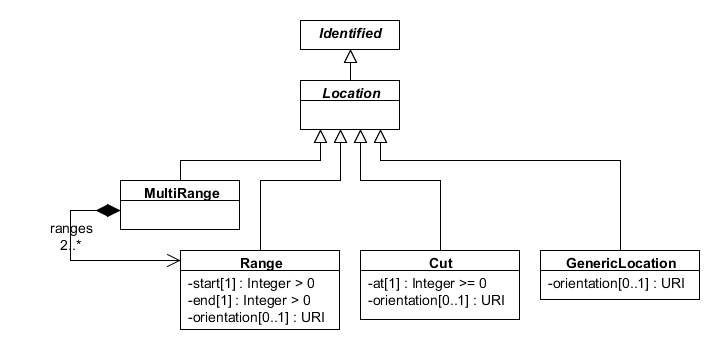
\includegraphics[scale=0.6]{uml/location}
\caption[]{Diagram of the \sbol{Location} class and its associated properties.}
\label{uml:location}
\end{center}
\end{figure} \todo{change diagram to reflect changes from SEP 41}

\subparagraph{The \sbolheading{orientation} property}
\label{sec:orientation}
The \sbol{orientation} property is OPTIONAL and has a data type of \sbol{URI}. All subclasses of \sbol{Location} share this property, which can be used to indicate how the region specified by the \sbol{SequenceFeature} and any associated double-stranded \sbol{Feature} is oriented on the \sbol{elements} of a \sbol{Sequence}  from their parent \sbol{Component}. \ref{tbl:orientation_types} provides a list of REQUIRED \sbol{orientation} \sbol{URI}s. If a \sbol{Location} object has an \sbol{orientation}, then it MUST come from \ref{tbl:orientation_types}.

\subparagraph{The \sbolheading{sequence} property}
\label{sec:sequence}
The \sbol{sequence} property is REQUIRED and MUST contain the \sbol{URI} of a \sbol{Sequence} object. All subclasses of \sbol{Location} share this property, which indicates which \sbol{Sequence} object referenced by the containing \sbol{Component} is referenced by the \sbol{Location}.

\begin{table}[ht]
  \begin{edtable}{tabular}{lp{3.75in}}
    \toprule
    \textbf{Orientation URI} & \textbf{Description} \\
    \midrule
    \url{http://sbols.org/v2\#inline} & The region specified by this \sbol{Location} is on the \sbol{elements} of a \sbol{Sequence}. \\
    \url{http://sbols.org/v2\#reverseComplement} & The region specified by this \sbol{Location} is on the reverse-complement translation of the \sbol{elements} of a \sbol{Sequence}. The exact nature of this translation depends on the \sbol{encoding} of the \sbol{Sequence}. \\
    \bottomrule
  \end{edtable}
  \caption{REQUIRED \sbol{URI}s for the \sbol{orientation} property}
  \label{tbl:orientation_types}
\end{table}


\paragraph{Range}
\label{sec:Range}
A \sbol{Range} object specifies a region via discrete, inclusive \sbol{start} and \sbol{end} positions that correspond to indices for characters in the \sbol{elements} \sbol{String} of a \sbol{Sequence}.

Note that the index of the first location is 1, as is typical practice in biology, rather than 0, as is typical practice in computer science.

\subparagraph{The \sbolheading{start} property}\label{sec:start}
The \sbol{start} property specifies the inclusive starting position of the \sbol{Range}. This property is REQUIRED and MUST contain an \sbol{Integer} value greater than zero.

\subparagraph{The \sbolheading{end} property}\label{sec:end}
The \sbol{end} property specifies the inclusive ending position of the \sbol{Range}. This property is REQUIRED and MUST contain an \sbol{Integer} value greater than zero. In addition, this \sbol{Integer} value MUST be greater than or equal to that of the \sbol{start} property.

\paragraph{Cut}
\label{sec:Cut}
The \sbol{Cut} class has been introduced to enable the specification of a region between two discrete positions.
This specification is accomplished using the \sbol{at} property, which specifies a discrete position that that corresponds to the index of a character in the \sbol{elements} \sbol{String} of a \sbol{Sequence} (except in the case when \sbol{at} is equal to zero---see below).

\subparagraph{The \sbolheading{at} property}
\label{sec:at}
The \sbol{at} property is REQUIRED and MUST contain an \sbol{Integer} value greater than or equal to zero. The region specified by the \sbol{Cut} is between the position specified by this property and the position that immediately follows it. When the \sbol{at} property is equal to zero, the specified region is immediately before the first discrete position or character in the \sbol{elements} \sbol{String} of a \sbol{Sequence}.


\paragraph{EntireSequence}
\label{sec:EntireSequence}
The \sbol{EntireSequence} class does not have any additional properties. Use of this class indicates that the linked Sequence describes the entirety of the \sbol{Component} or \sbol{Feature} parent of this Location object.

\subparagraph{The \sbolheading{order} property}
\label{sec:order}


\subsubsection{Constraint}
\label{sec:Constraint}
The \sbol{Constraint} class can be used to assert restrictions on the relationships of pairs of \sbol{Feature} objects contained by the same parent \sbol{Component}.
Uses of this class include expressing containment (e.g., a plasmid transformed into a chassis strain), identity mappings (e.g., replacing a placeholder value with a complete definition), and expressing relative, sequence-based positions (e.g., the ordering of features within a template).
Each \sbol{Constraint} includes the \sbol{restriction}, \sbol{subject}, and \sbol{object} properties.

\begin{figure}[ht]
\begin{center}
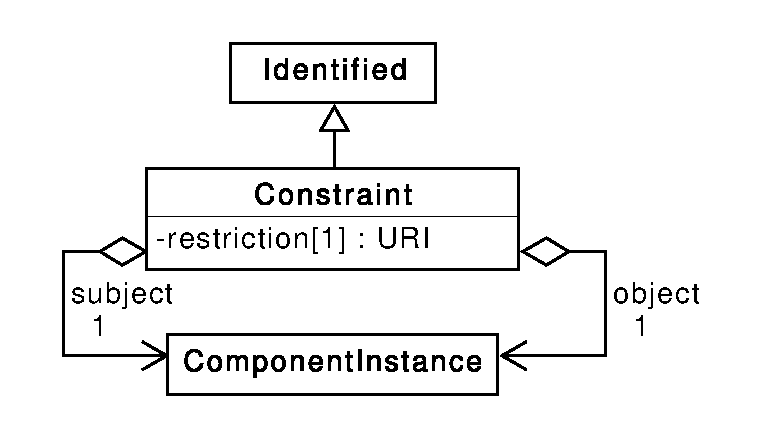
\includegraphics[scale=0.6]{uml/constraint}
\caption[]{Diagram of the \sbol{Constraint} class and its associated properties.}
\label{uml:sequence_constraint}
\end{center}
\end{figure}

\subparagraph{The \sbolheading{subject} property}\label{sec:subject}
The \sbol{subject} property is REQUIRED and MUST contain a \sbol{URI} that refers to a \sbol{Feature} contained by the same parent \sbol{Component} that contains the \sbol{Constraint}.

\subparagraph{The \sbolheading{object} property}\label{sec:object}
The \sbol{object} property is REQUIRED and MUST contain a \sbol{URI} that refers to a \sbol{Feature} contained by the same parent \sbol{Component} that contains the \sbol{Constraint}. This \sbol{Feature} MUST NOT be the same \sbol{Feature} that the \sbol{Constraint} refers to via its \sbol{subject} property.

\subparagraph{The \sbolheading{restriction} property}\label{sec:restriction}

The \sbol{restriction} property is REQUIRED and has a data type of \sbol{URI}. 
This property MUST indicate the type of restriction on the locations, orientations, or identities of the \sbol{subject} and \sbol{object} \sbol{Feature} objects in relation to each other. 
The \sbol{URI} value of this property SHOULD come from the RECOMMENDED \sbol{URI}s in \ref{tbl:restriction_types_identity}, \ref{tbl:restriction_types_topology}, and \ref{tbl:restriction_types_sequence}.

% identify and orientation
\begin{table}[ht]
  \begin{edtable}{tabular}{lp{3.25in}}
    \toprule
    \textbf{Restriction URI} & \textbf{Description} \\
    \midrule
    % identity relations
	\url{http://sbols.org/v3#verifyIdentical}  & The \sbol{instanceOf} properties of the \sbol{subject} and \sbol{object} \sbol{Feature} objects MUST refer to the same \sbol{Component}.  \emph{Example: a promoter included via two different subsystems must be the identical.} \\
	\url{http://sbols.org/v3\#differentFrom} & The \sbol{instanceOf} property of the \sbol{subject} \sbol{Feature} MUST NOT refer to the same \sbol{Component} as that of the \sbol{object} \sbol{Component}. \emph{Example: two fluorescent reporters must be different.}\\
	\url{http://sbols.org/v3#replaces} &	In the context of the parent object of the \sbol{Constraint}, information about the \sbol{subject} should be used in place of all instances of the \sbol{object}. \emph{Example: the J23101 promoter replaces a generic promoter.} \\
    
    % orientation relations
	\url{http://sbols.org/v3\#sameOrientationAs} & The \sbol{subject} and \sbol{object} \sbol{Component} objects MUST have the same orientation. \emph{Example: a promoter has the same orientation as the coding sequence it controls.}\\
	\url{http://sbols.org/v2\#oppositeOrientationAs} & The \sbol{subject} and \sbol{object} \sbol{Component} objects MUST have opposite orientations. \emph{Example: a promoter has the opposite orientation as an invertase-activated coding sequence it controls.}\\

    \bottomrule
  \end{edtable}
  \caption{RECOMMENDED \sbol{URI}s for expressing identity and orientation with the \sbol{restriction} property.}
  \label{tbl:restriction_types_identity}
\end{table}

    % topology relations
\begin{table}[ht]
  \begin{edtable}{tabular}{lp{3.25in}}
    \toprule
    \textbf{Restriction URI} & \textbf{Description} \\
    \midrule
	\url{http://sbols.org/v3#isDisjointFrom}	& The \sbol{subject} and \sbol{object} do not overlap in space. \emph{Example: a plasmid is disjoint from a chromosome.} \\
	\url{http://sbols.org/v3#strictlyContains} &	The \sbol{subject} entirely contains the \sbol{object}: they do not share a boundary. \emph{Example: a cell contains a plasmid} \\
	\url{http://sbols.org/v3#contains} &	The \sbol{subject} contains the \sbol{object} and they might or might not share a boundary (i.e., union of {\tt strictlyContains}, {\tt equals}, and {\tt covers}. \emph{Example: a cell contains a protein that may or may not bind to its membrane.} \\
	\url{http://sbols.org/v3#equals} &	The \sbol{subject} and \sbol{object} occupy the same location in space. \emph{Example: a small molecule is distributed throughour an entire sample.} \\
	\url{http://sbols.org/v3#meets} &	The \sbol{subject} and \sbol{object} are connected at a shared boundary. \emph{Example: two strains of adherent cells meet at their membranes.} \\
	\url{http://sbols.org/v3#covers} &	The \sbol{subject} contains the \sbol{object} but also shares a boundary. \emph{Example: a cell covers its transmembrane proteins.} \\
	\url{http://sbols.org/v3#overlaps} &	The \sbol{subject} and \sbol{object} overlap in space, but portions of each are outside of the other. \emph{Example: a transmembrane protein overlaps the cell membrane.} \\
    \bottomrule
  \end{edtable}
  \caption{RECOMMENDED \sbol{URI}s for expressing topological relations with the \sbol{restriction} property.}
  \label{tbl:restriction_types_topology}
\end{table}

\begin{table}[ht]
  \begin{edtable}{tabular}{lp{3.25in}}
    \toprule
    \textbf{Restriction URI} & \textbf{Description} \\
    \midrule
    % linear relations
	\url{http://sbols.org/v3#precedes} &	The start of the location for \sbol{subject} is less than the start of the location for \sbol{object} (i.e., union of \sbol{strictlyPrecedes}, \sbol{meets}, and \sbol{overlaps}). 
	\emph{Example: a promoter precedes a ribosome entry site, but the exact boundary between the two will be determined by sequence optimization and assembly planning}. \\
	
	\url{http://sbols.org/v3#strictlyPrecedes} &	The end of the location for \sbol{subject} is less than the start of the location for \sbol{object}. 
	\emph{Example: a promoter strictly precedes a terminator (with a CDS between them).} \\
	
	\url{http://sbols.org/v3#meets} &	The end of the location for \sbol{subject} is equal to the start of the location for \sbol{object}. 
	Note: this is a stronger interpretation of {\tt meets} from \ref{tbl:restriction_types_topology} in the context of a linear sequence.
	\emph{Example: the 3' region adjacent to a blunt restriction site meets the 5' region adjacent to the site.} \\
	
	\url{http://sbols.org/v3#overlaps} &	The start of the location for \sbol{subject} is before the start of the location for \sbol{object} and the end of the location for \sbol{subject} is before the end of the location for \sbol{object}. 
	Note: this is a stronger interpretation of {\tt overlaps} from \ref{tbl:restriction_types_topology} in the context of a linear sequence.
	\emph{Example: two oligos in a Gibson assembly plan} \\
	
	\url{http://sbols.org/v3#contains} &	The start of the location for \sbol{subject} is less than or equal to the start of the location for \sbol{object} and the end of the location for \sbol{subject} is greater than or equal to the end of the location for \sbol{object} (i.e., union of {\tt strictlyContains}, {\tt equals}, {\tt finishes}, and {\tt starts}). 
	Note: this is a stronger interpretation of {\tt contains} from \ref{tbl:restriction_types_topology} in the context of a linear sequence.
	\emph{Example: a composite part contains a promoter} \\
	
	\url{http://sbols.org/v3#strictlyContains} &	The start of the location for \sbol{subject} is before the start of the location for \sbol{object} and the end of the location for \sbol{subject} is after the end of the location for \sbol{object}. 
	Note: this is a stronger interpretation of {\tt strictlyContains} from \ref{tbl:restriction_types_topology} in the context of a linear sequence.
	\emph{Example: an RNA transcript strictly contains an intron.} \\
	
	\url{http://sbols.org/v3#equals} &	The start and end of the location for \sbol{subject} are equal to the start and end of the location for \sbol{object}. 
	Note: this is a stronger interpretation of {\tt equals} from \ref{tbl:restriction_types_topology} in the context of a linear sequence.
	\emph{Example: the transcribed region of a CDS part equals the entire part.} \\
	
	\url{http://sbols.org/v3#finishes} &	The start of the location for \sbol{subject} is after the start of the location for \sbol{object} and the end of the location for \sbol{subject} is equal to the end of the location for \sbol{object}. 
	\emph{Example: a terminator finishes an expression cassette.} \\
	
	\url{http://sbols.org/v3#starts} &	The start of the location for \sbol{subject} is equal to the start of the location for \sbol{object} and the end of the location for \sbol{subject} is before the end of the location for \sbol{object}. 
	\emph{Example: a promoter starts an expression cassette.} \\
    \bottomrule
  \end{edtable}
  \caption{RECOMMENDED \sbol{URI}s for expressing sequential relations with the \sbol{restriction} property.}
  \label{tbl:restriction_types_sequence}
\end{table}



\subsection{Model}
\label{sec:Model}

\begin{figure}[ht]
\begin{center}
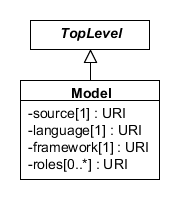
\includegraphics[scale=0.6]{uml/model}
\caption[]{Diagram of the \sbol{Model} class and its associated properties.}
\label{uml:model}
\end{center}
\end{figure}

The purpose of the \sbol{Model} class is to serve as a placeholder for an external computational model and provide additional meta-data to enable better reasoning about the contents of this model.
In this way, there is minimal duplication of standardization efforts and users of SBOL can formalize the function of a \sbol{Component} in the language of their choice.

The meta-data provided by the \sbol{Model} class include the following properties: the \sbolmult{source:M}{source} or location of the actual content of the model, the \sbol{language} in which the model is implemented, and the model's \sbol{framework}.

\subparagraph{ The \sbolheading{source} property}\label{sec:source:M}
The \sbolmult{source:M}{source} property is REQUIRED and MUST contain a \sbol{URI} reference to the source file for a model.

\subparagraph{ The \sbolheading{language} property}\label{sec:language}
The \sbol{language} property is REQUIRED and MUST contain a \sbol{URI} that specifies the language in which the model is implemented. It is RECOMMENDED that this \sbol{URI} refer to a term from the EMBRACE Data and Methods (EDAM) ontology. \ref{tbl:model_types} provides a list of terms from this ontology and their \sbol{URI}s. If the \sbol{language} property of a \sbol{Model} is well-described by one these terms, then it MUST contain the \sbol{URI} for this term as its value.

\begin{table}[ht]
  \begin{edtable}{tabular}{ll}
    \toprule
    \textbf{Model Language} & \textbf{URI for EDAM Term} \\
    \midrule
    SBML  & \url{http://identifiers.org/edam/format_2585}\\
    CellML		 & \url{http://identifiers.org/edam/format_3240}\\
    BioPAX    & \url{http://identifiers.org/edam/format_3156}\\
    \bottomrule
  \end{edtable}
  \caption{Terms from the EDAM ontology to specify the \sbol{language} property of a \sbol{Model}.}
  \label{tbl:model_types}
\end{table}


\subparagraph{ The \sbolheading{framework} property}\label{sec:framework}
The \sbol{framework} property is REQUIRED and MUST contain a \sbol{URI} that specifies the framework in which the model is implemented.
It is RECOMMENDED this \sbol{URI} refer to a term from the modeling framework branch of the SBO when possible. A few suggested modeling frameworks and their corresponding \sbol{URI}s are shown in \ref{tbl:model_frameworks}. If the \sbol{framework} property of a \sbol{Model} is well-described by one these terms, then it MUST contain the \sbol{URI} for this term as its value.

\begin{table}[ht]
  \begin{edtable}{tabular}{ll}
    \toprule
    \textbf{Framework} & \textbf{URI for SBO Term} \\
    \midrule
    Continuous  & \url{http://identifiers.org/biomodels.sbo/SBO:0000062}\\
    Discrete & \url{http://identifiers.org/biomodels.sbo/SBO:0000063}\\
    \bottomrule
  \end{edtable}
  \caption{SBO terms to specify the \sbol{framework} property of a \sbol{Model}.}
  \label{tbl:model_frameworks}
\end{table}

\subsection {Collection}
\label{sec:Collection}
The \sbol{Collection} class is a class that groups together a set of \sbol{TopLevel} objects that have something in common.
Some examples of \sbol{Collection} objects:
\begin{itemize}
\item Results of a query to find all \sbol{Component} objects in a repository that function as promoters.
\item A set of \sbol{Component} objects representing a library of genetic logic gates.
\item A \sbol{Component} for a complex design, and all of the \sbol{Component}, \sbol{Component},\\ \sbol{Sequence}, and \sbol{Model} objects used to provide its full specification.
\end{itemize}

\begin{figure}[ht]
\begin{center}
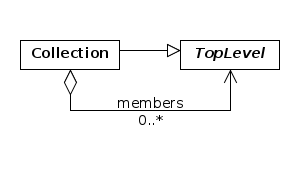
\includegraphics[scale=0.6]{uml/collection}
\caption[]{Diagram of the \sbol{Collection} class and its associated properties.}
\label{uml:collection}
\end{center}
\end{figure}

\subparagraph{The \sbolheading{members} property}\label{sec:members}
The \sbol{members} property of a \sbol{Collection} is OPTIONAL and MAY contain a set of \sbol{URI} references to zero or more \sbol{TopLevel} objects.

\subsection{Namespace}
\label{sec:Namespace}
The \sbol{Namespace} class is a subclass of \sbol{Collection} and is used to define \sbol{member} entities that share the same prefix in their \sbol{identity} properties. All linked objects must have a URI prefix matching the identity of a \sbol{Namespace} object. 

\begin{figure}[ht]
\begin{center}
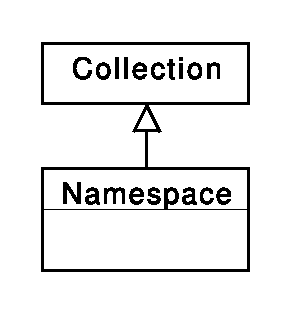
\includegraphics[scale=0.6]{uml/namespace}
\caption[]{\sbol{Namespace} is a special case of \sbol{Collection}.}
\label{uml:namespace}
\end{center}
\end{figure}

\subsection{CombinatorialDerivation}
\label{sec:CombinatorialDerivation}

The purpose of the \sbol{CombinatorialDerivation} class is to specify combinatorial genetic designs without having to specify every possible design variant. For example, a \sbol{CombinatorialDerivation} can be used to specify a library of reporter gene variants that include different promoters and RBSs without having to specify a \sbol{Component} for every possible combination of promoter, RBS, and CDS in the library. \sbol{Component} objects that realize a \sbol{CombinatorialDerivation} can be derived in accordance with the class properties \sbol{template}, \\
\sbol{variableComponents}, and \sbol{strategy} (see \ref{uml:combinatorial_derivation}).

\begin{figure}[ht]
\begin{center}
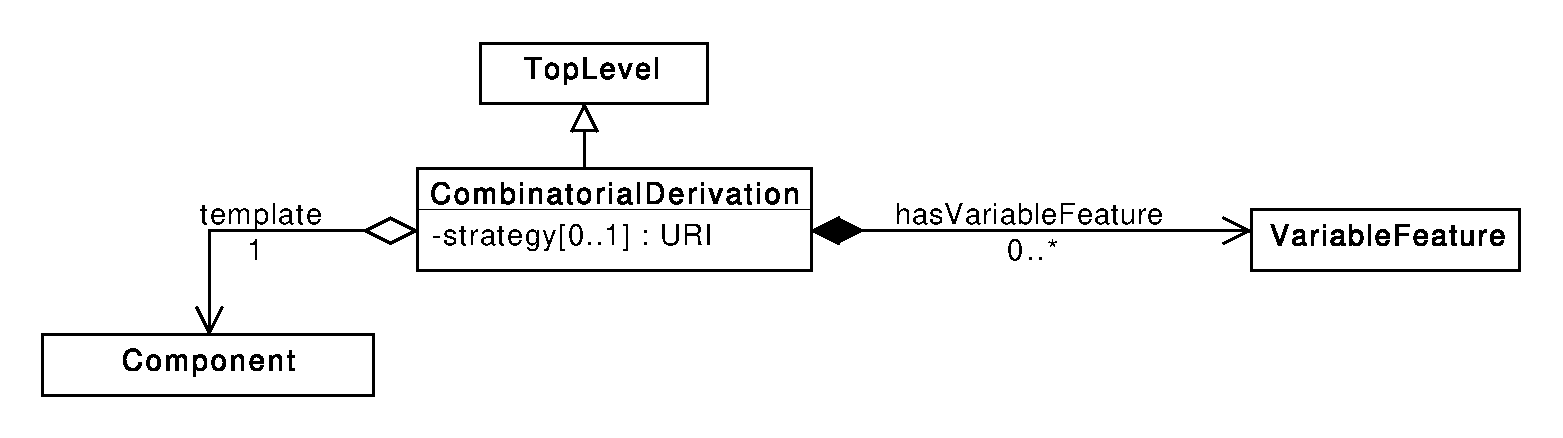
\includegraphics[scale=0.6]{uml/combinatorial_derivation}
\caption[]{Diagram of the \sbol{CombinatorialDerivation} class and its associated properties.}
\label{uml:combinatorial_derivation}
\end{center}
\end{figure}

\subparagraph{ The \sbolheading{template} property}\label{sec:template}

The \sbol{template} property is REQUIRED and MUST contain a URI that refers to a \sbol{Component}. 
This \sbol{Component} is expected to serve as a template for the derivation of new \sbol{Component} objects. 
Consequently, its \sbol{feature}s property SHOULD contain one or more \sbol{Feature} objects that describe its substructure (referred to hereafter as template \sbol{Feature} objects), and its \sbol{constraint} property MAY also contain one or more \sbol{Constraint} objects that constrain this substructure.

When a \sbol{Component} is derived in accordance with a \sbol{CombinatorialDerivation}, the \sbol{prov:wasDerivedFrom} property of the derived \sbol{Component} SHOULD refer to the \sbol{CombinatorialDerivation}. When multiple \sbol{Component} objects are derived in accordance with the same \sbol{CombinatorialDerivation}, they MAY be referred to by the \sbol{members} property of a \sbol{Collection}, in which case the \sbol{prov:wasDerivedFrom} property of the \sbol{Collection} SHOULD also refer to this \sbol{CombinatorialDerivation}.

If the \sbolmult{types:CD}{types} property of the template \sbol{Component} contains one or more URIs, then the \sbolmult{types:CD}{types} property of the derived \sbol{Component} SHOULD also contain those URIs. The same holds true for the \sbolmult{roles:CD}{roles} properties of these \sbol{Component} objects.

\subparagraph{ The \sbolheading{variableComponents} property}\label{sec:variableComponents}

The \sbol{variableComponents} property is OPTIONAL and MAY contain a set of \sbol{VariableComponent} objects. These \sbol{VariableComponent} objects are expected to denote the choices available when deriving the substructure of a new \sbol{Component} in accordance with a \sbol{CombinatorialDerivation}. The \sbol{variableComponents} property MUST NOT contain two or more \sbol{VariableComponent} objects that refer to the same template \sbol{Feature} via their \sbol{variable} properties.

If the \sbol{variable} property of one of these \sbol{VariableComponent} objects refers to a template \sbol{Feature}, then the \sbol{feature}s property of the derived \sbol{Component} SHOULD contain as many \sbol{Feature} objects derived from the template \sbol{Feature} as specified by the \sbol{operator} property of the \sbol{VariableComponent} (see \ref{tbl:operator}). In addition, the \sbol{instanceOf} properties of these derived \sbol{Feature} objects MUST refer to \sbol{Component} objects specified by the \sbol{variants}, \sbol{variantCollections}, or \sbol{variantDerivations} property of the \sbol{VariableComponent}.

If no \sbol{variable} property of one of these \sbol{VariableComponent} objects refers to a template \sbol{Feature}, then the \sbol{feature}s property of the derived \sbol{Component} SHOULD contain exactly one \sbol{Feature} with a \sbol{prov:wasDerivedFrom} property that refers to the template \sbol{Feature}. The \sbol{instanceOf} property of this derived \sbol{Feature} MUST refer to the \sbol{Component} referred to by the \sbol{instanceOf} property of the template \sbol{Feature}.

Finally, all of these derived \sbol{Feature} objects MUST follow the \sbol{restriction} properties of any \\
\sbol{Constraint} objects that refer to their corresponding template \sbol{Feature} objects.

\subparagraph{ The \sbolheading{strategy} property}\label{sec:strategy}
The \sbol{strategy} property is OPTIONAL and has a data type of URI. \ref{tbl:strategy} provides a list of REQUIRED \sbol{strategy} URIs. If the \sbol{strategy} property is not empty, then it MUST contain a URI from \ref{tbl:strategy}. This property recommends how many \sbol{Component} objects a user SHOULD derive from the template \sbol{Component}.


\begin{table}[ht]
  \begin{edtable}{tabular}{lp{4in}}
    \toprule
    \textbf{Strategy URI} & \textbf{Description} \\
    \midrule
    \url{http://sbols.org/v2#enumerate}  &  A user SHOULD derive all possible \sbol{Component} objects specified by the \sbol{CombinatorialDerivation}. \\
        \url{http://sbols.org/v2#sample}  & A user SHOULD derive a subset of all possible \sbol{Component} objects specified by \sbol{CombinatorialDerivation}. The manner in which this subset is chosen is for the user to decide. \\
    \bottomrule
  \end{edtable}
  \caption{REQUIRED \sbol{URI}s for the \sbol{strategy} property.}
  \label{tbl:strategy}
\end{table}


\subsubsection{VariableComponent}
\label{sec:VariableComponent}

The \sbol{VariableComponent} class can be used to specify a choice of \sbol{Component} objects for any new \sbol{SubComponent} derived from a template \sbol{SubComponent} in the template \sbol{Component}. This specification is made using the class properties \sbol{variable}, \sbol{variants}, \sbol{variantCollections}, and \sbol{variantDerivations} (see \ref{uml:variable_component}). While the \sbol{variants}, \sbol{variantCollections}, and \sbol{variantDerivations} properties are OPTIONAL, at least one of them MUST NOT be empty. If these properties contain duplicate URIs, then they SHOULD be treated as a single URI for the purpose of selection. For example, if the \sbol{variants} property contains two copies of URI $A$ and one copy of URI $B$, $A$ SHOULD NOT be selected twice during enumeration, and it SHOULD NOT be selected twice as much as $B$ during sampling.

\begin{figure}[ht]
\begin{center}
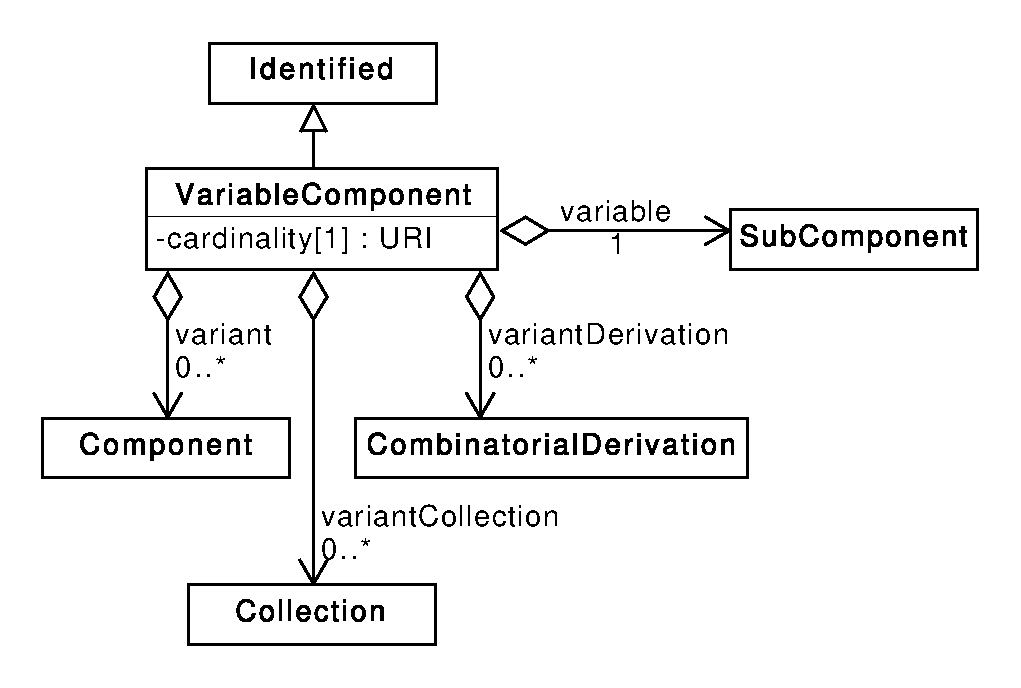
\includegraphics[scale=0.6]{uml/variable_component}
\caption[]{Diagram of the \sbol{VariableComponent} class and its associated properties.}
\label{uml:variable_component}
\end{center}
\end{figure}

\subparagraph{ The \sbolheading{variable} property}\label{sec:variable}

The \sbol{variable} property is REQUIRED and MUST contain a URI that refers to a template \sbol{SubComponent} in the template \sbol{Component}. If the \sbol{prov:wasDerivedFrom} property of a \sbol{SubComponent} refers to this template \sbol{SubComponent}, then the \sbol{instanceOf} property of the derived \sbol{SubComponent} MUST refer to either (1) a \sbol{Component} referred to by the \sbol{variants} property of the \sbol{VariableComponent}, (2) a \sbol{Component} from a \sbol{Collection} referred to by the \sbol{variantCollections} property of the \sbol{VariableComponent}, or (3) a \sbol{Component} derived from a \sbol{CombinatorialDerivation} referred to by the \sbol{variantDerivations} property of the \sbol{VariableComponent}.

If the \sbolmult{roles:CD}{roles} property of the template \sbol{SubComponent} contains one or more URIs, then the \sbolmult{roles:CD}{roles} property of the derived \sbol{SubComponent} SHOULD also contain those URIs.

\subparagraph{ The \sbolheading{variants} property}\label{sec:variants}

The \sbol{variants} property is OPTIONAL and MAY contain zero or more URIs that each refer to a \sbol{Component}. This property specifies individual \sbol{Component} objects to serve as options when deriving a new\\
\sbol{SubComponent} from the template \sbol{SubComponent}.

\subparagraph{ The \sbolheading{variantCollections} property}\label{sec:variantCollections}

The \sbol{variantCollections} property is OPTIONAL and MAY contain zero or more URIs that each refer to a\\
\sbol{Collection}. The \sbol{members} property of each \sbol{Collection} referred to in this way MUST NOT be empty. This property enables the convenient specification of existing groups of \sbol{Component} objects to serve as options when deriving a new \sbol{SubComponent} from the template \sbol{SubComponent}.

\subparagraph{ The \sbolheading{variantDerivations} property}\label{sec:variantDerivations}

The \sbol{variantDerivations} property is OPTIONAL and MAY contain zero or more URIs that each refer to a\\ \sbol{CombinatorialDerivation}. This property enables the convenient specification of \sbol{Component} objects derived in accordance with another \sbol{CombinatorialDerivation} to serve as options when deriving a new \sbol{SubComponent} from the template \sbol{SubComponent}. The \sbol{variantDerivations} property of a \sbol{VariableComponent} MUST NOT refer to the \sbol{CombinatorialDerivation} that contains this \sbol{VariableComponent}. Furthermore, \sbol{VariableComponent} objects MUST NOT form a cyclical chain of references via their \sbol{variantDerivations} properties and the\\ \sbol{CombinatorialDerivation} objects that contain them. For example, consider the \sbol{VariableComponent} objects A and B and the \sbol{CombinatorialDerivation} objects X and Y. The reference chain X contains A, A has variant derivation Y, Y contains B, and B has variant derivation X is cyclical.

\subparagraph{ The \sbolheading{operator} property}\label{sec:operator}

The \sbol{operator} property is REQUIRED and has a data type of URI. This property specifies how many \sbol{SubComponent} objects SHOULD be derived from the template \sbol{SubComponent} during the derivation of a new \sbol{Component}. The URI value of this property MUST come from the URIs provided in~\ref{tbl:operator}.


\begin{table}[ht]
  \begin{edtable}{tabular}{lp{4in}}
    \toprule
    \textbf{Operator URI} & \textbf{Description} \\
    \midrule
    \url{http://sbols.org/v2#zeroOrOne} & No more than one \sbol{SubComponent} in the derived \sbol{Component} SHOULD have a \sbol{prov:wasDerivedFrom} property that refers to the template \sbol{SubComponent}. \\
        \url{http://sbols.org/v2#one} & Exactly one \sbol{SubComponent} in the derived \sbol{Component} SHOULD have a \sbol{prov:wasDerivedFrom} property that refers to the template \sbol{SubComponent}. \\
\url{http://sbols.org/v2#zeroOrMore} & Any number of \sbol{SubComponent} objects in the derived \sbol{Component} MAY have \sbol{prov:wasDerivedFrom} properties that refer to the template \sbol{SubComponent}. \\
\url{http://sbols.org/v2#oneOrMore} & At least one \sbol{SubComponent} in the derived \sbol{Component} SHOULD have a \sbol{prov:wasDerivedFrom} property that refers to the template \sbol{SubComponent}. \\
    \bottomrule
  \end{edtable}
  \caption{REQUIRED \sbol{URI}s for the \sbol{operator} property.}
  \label{tbl:operator}
\end{table}


\subsection{Implementation}
\label{sec:Implementation}


An \sbol{Implementation} represents an instance of a synthetic biological construct, and describes the build phase of a design-built-test-learn workflow. Importantly, an \sbol{Implementation} can be associated with a laboratory sample that was already built, or that is to be built in the future. An \sbol{Implementation} can also represent virtual and simulated instances.  An \sbol{Implementation} may be linked back to its original design (either a \sbol{Component} or \sbol{Component}) using the \sbol{prov:wasDerivedFrom} property inherited from the \sbol{Identified} superclass. An \sbol{Implementation} may also link to a \sbol{Component} or \sbol{Component} that specifies its realized structure and/or function.
% as described in Section2.1.1.

\begin{figure}[ht]
\begin{center}
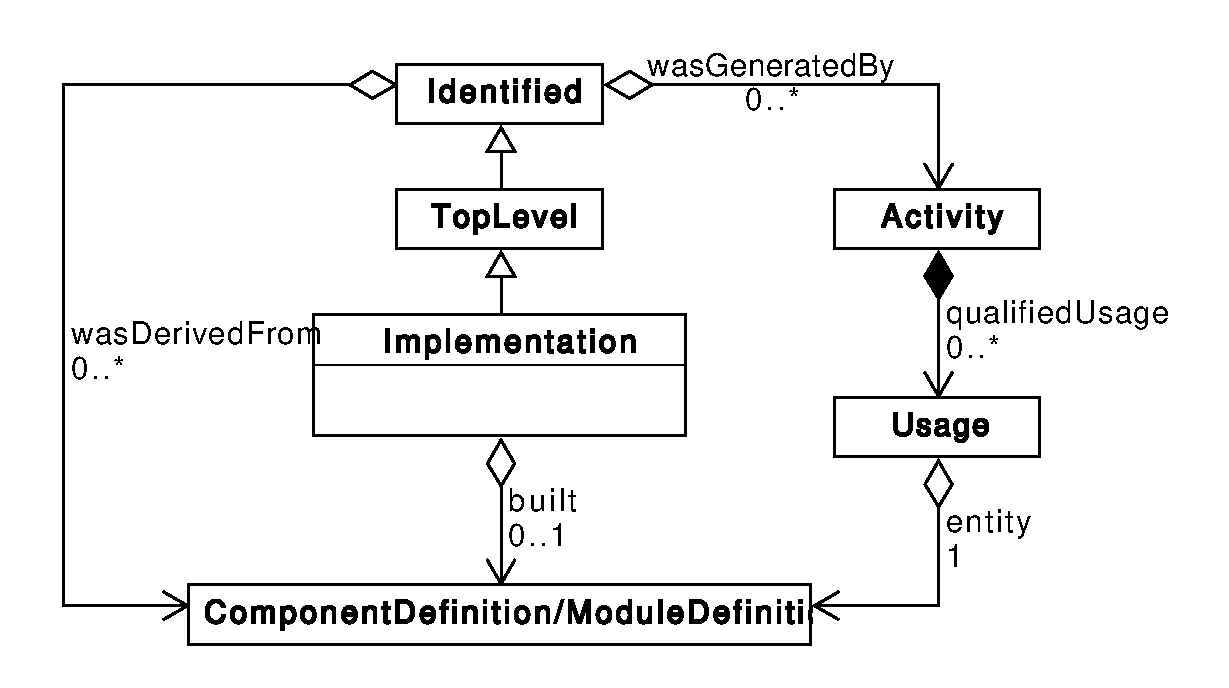
\includegraphics[scale=0.5]{uml/implementation}
\caption[]{Diagram of the \sbol{Implementation} class and its associated properties.}
\label{uml:implementation}
\end{center}
\end{figure}

\subparagraph{ The \sbolheading{built} property}\label{sec:built}
The \sbol{built} property is OPTIONAL and MAY contain a URI that MUST refer to a \sbol{TopLevel} object that is either a \sbol{Component} or \sbol{Component}. This \sbol{Component} or \sbol{Component} is intended to describe the actual physical structure and/or functional behavior of the \sbol{Implementation}. When the built property refers to a \sbol{Component} or \sbol{Component} that is also linked to the \sbol{Implementation} via PROV-O properties such as \sbol{prov:wasDerivedFrom} (see \ref{sec:provenance}), it can be inferred that the actual structure and/or function of the \sbol{Implementation} matches its original design. When the \sbol{built} property refers to a different \sbol{Component} or \sbol{Component}, it can be inferred that the \sbol{Implementation} has deviated from the original design. For example, the latter could be used to document when the DNA sequencing results for an assembled construct do not match the original target sequence.



\subsection{Attachment}
\label{sec:Attachment}

\begin{figure}[ht]
\begin{center}
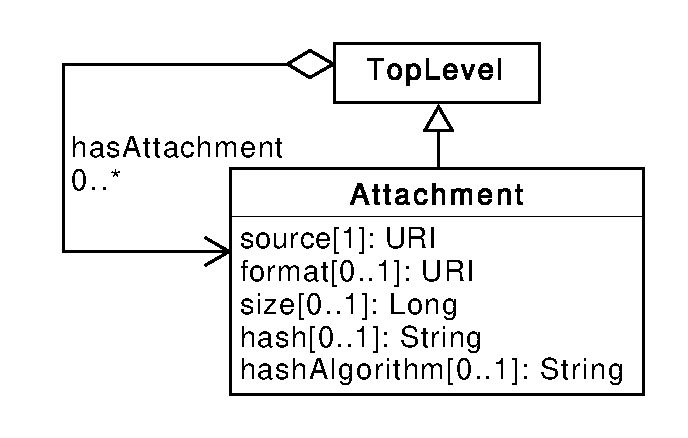
\includegraphics[scale=0.6]{uml/attachment}
\caption[]{Diagram of the \sbol{Attachment} class and its associated properties.}
\label{uml:attachment}
\end{center}
\end{figure}

The purpose of the \sbol{Attachment} class is to serve as a general container for data files, especially experimental data files.
It provides a means for linking files and metadata to SBOL designs.

The meta-data provided by the \sbol{Attachment} class include the following properties: the \sbolmult{source:A}{source} or location of the actual file of the attachment, the \sbol{format} of the file, the \sbol{size} of the file, and the \sbol{hash} for the file.

\subparagraph{ The \sbolheading{source} property}\label{sec:source:A}
The \sbolmult{source:A}{source} property is REQUIRED and MUST contain a \sbol{URI} reference to the source file.

\subparagraph{ The \sbolheading{format} property}\label{sec:format}
The \sbol{format} property is OPTIONAL and MAY contain a \sbol{URI} that specifies the format of the attached file. It is RECOMMENDED that this \sbol{URI} refer to a term from the EMBRACE Data and Methods (EDAM) ontology.

\subparagraph{ The \sbolheading{size} property}\label{sec:size}
The \sbol{size} property is OPTIONAL and MAY contain a long indicating the file size in bytes.

\subparagraph{ The \sbolheading{hash} property}\label{sec:hash}
The \sbol{hash} property is OPTIONAL and MAY contain a SHA-1 hash of the file contents represented as a hexadecimal digest.

\subsection{ExperimentalData}
\label{sec:ExperimentalData}


\begin{figure}[ht]
\begin{center}
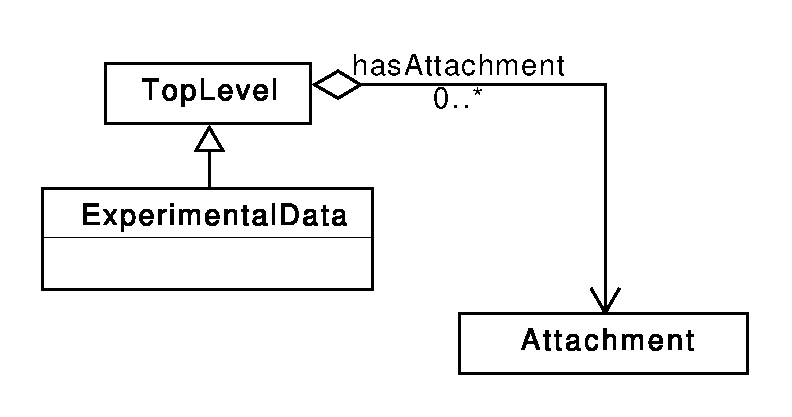
\includegraphics[scale=0.6]{uml/experimental_data}
\caption[]{Diagram of the \sbol{ExperimentalData} class and its associated properties.}
\label{uml:experimental_data}
\end{center}
\end{figure}

The purpose of the \sbol{ExperimentalData} class is to aggregate links to experimental data files. An \sbol{ExperimentalData} is typically associated with a single sample, lab instrument, or experimental condition and can be used to describe the output of the test phase of a design-build-test-learn workflow. For an example of the latter, see \ref{images:design-build-test-learn}.

As shown in \ref{uml:experimental_data}, the \sbol{ExperimentalData} class aggregates links to experimental data files using the OPTIONAL \sbol{hasAttachment} property that it inherits from the \sbol{TopLevel} class.

\subsection{Experiment}
\label{sec:Experiment}


\begin{figure}[ht]
\begin{center}
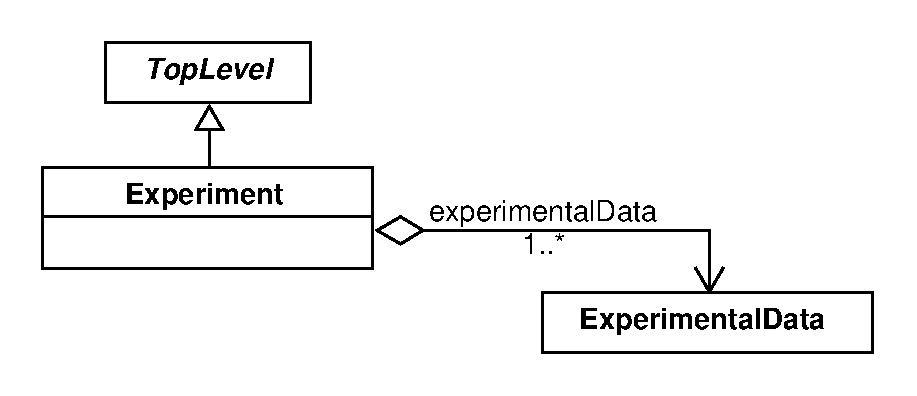
\includegraphics[scale=0.6]{uml/experiment}
\caption[]{Diagram of the \sbol{Experiment} class and its associated properties.}
\label{uml:experiment}
\end{center}
\end{figure}

The purpose of the \sbol{Experiment} class is to aggregate experimental data sets for subsequent analysis, usually in accordance with an experimental design. 

As shown in \ref{uml:experimental_data}, the \sbol{Experiment} class aggregates \sbol{ExperimentalData} objects via the \sbol{experimentalData} property.

\subparagraph{ The \sbolheading{experimentalData} property}\label{sec:experimentalData}
The \sbol{experimentalData} property is OPTIONAL and MAY contain a set of \sbol{URI} references to \sbol{ExperimentalData} objects. The same \sbol{ExperimentalData} MAY be referred to by more than one \sbol{Experiment} in this way.

\subsection{Annotation and Extension of SBOL}
\label{sec:Annotations}

SBOL intentionally does not attempt to describe how all types of biological design data should be captured, since many of these data types (e.g., biological context and design performance metrics) are already covered by other standards, or lack a clear consensus on their proper representation. In addition, some types of biological data are not directly relevant to design and are therefore outside of the scope of SBOL.

SBOL is built upon the Resource Description Framework (RDF), and therefore can be used in conjunction with complementary standards as described in \autoref{sec:complementaryStandards}.  For example, use of the PROV-O ontology is recommended to capture provenance \autoref{sec:provenance}.  Additionally, user-defined RDF can be used in conjunction with SBOL objects to capture custom application-specific information which does not yet have a standardized representation.  This annotation and extension mechanism is designed to enable new types of data to be easily incorporated into the SBOL standard once there is community consensus on their proper representation.

Several methods are supported for connecting the SBOL data model with other types of application-specific data:

\begin{itemize}
\item Custom data can be added to an SBOL object by annotating that object with non-conflicting properties. These properties could contain \sbol{literal} data types such as \sbol{String}s or \sbol{URI}s that require a resolution mechanism to obtain external data. An example is annotating a \sbol{Component} with  a property that contains a \sbol{String} description and \sbol{URI} for the parts registry from which its source data was originally imported.
\item Custom data in the form of independent objects can be participate in the SBOL data model if they are assigned one of the SBOL types \sbol{Identified} or \sbol{TopLevel}.  An example is an RDF object that is annotated such that it represents a data sheet that describes the performance of a \sbol{Component} in a particular context.
\item Finally, just as custom objects can be embedded in an  SBOL document, external documents can embed or refer to SBOL objects. Support for this last case is not explicitly provided in this specification. Rather, this case depends on the external non-SBOL system managing its relationship to SBOL and data serialized in RDF, and is included here for completeness.
\end{itemize}

\subsubsection{Annotating SBOL objects}
% whole set of labels for the properties defined herein
\label{sec:qName}
\label{sec:QName}
\label{sec:value}
\label{sec:Annotation}
\label{sec:AnnotationValue}
\label{sec:NestedAnnotations}
\label{sec:nestedQName}
\label{sec:nestedURI}

Each \sbol{Identified} object MAY be annotated with application-specific properties, which MUST be labelled using RDF predicates outside of the SBOL namespace.  Additionally, application-specific types may be used in conjunction with the SBOL data model. These application-specific types MUST have two \sbol{rdf:type} properties: one type outside of the SBOL namespace AND an additional SBOL type of either:

\begin{itemize}
  \item \sbol{TopLevel}, if the object is to be considered an SBOL top level (i.e., not owned by another object)
  \item \sbol{Identified}, if the object is not to be considered an SBOL top level (i.e., is owned by another object)
\end{itemize}

As with SBOL \sbol{TopLevel} objects, custom \sbol{TopLevel} objects MAY include the properties \sbol{displayId}, \sbol{name},\\ \sbol{description}, etc. 

\section{Mapping Between SBOL 1.1 and SBOL 2.x}
\label{sec:mapping}

\ref{SBOL1TO2} depicts the mapping of SBOL 1.1 classes to SBOL 2.x classes, indicating corresponding classes/properties by color.
The SBOL 2.x \sbol{Model} and \sbol{CompenentDefinition} classes have no SBOL 1.1 equivalent, and thus are not shown.
In particular:
\begin{itemize}
\item SBOL 1.1 \external{Collection} objects containing \external{DnaComponent} objects map to SBOL 2.x \sbol{Collection} objects that contain \sbol{CompenentDefinition} objects with DNA \sbolmult{types:CD}{types} properties.
\item SBOL 1.1 \external{DnaComponent} objects maps to SBOL 2.x \sbol{CompenentDefinition} objects with DNA \sbolmult{types:CD}{types} properties.
\item SBOL 1.1 \external{DnaSequence} objects maps to an SBOL 2.x \sbol{Sequence} objects with \external{IUPAC DNA} \sbol{encoding} properties.
\item SBOL 1.1 \external{SequenceAnnotation} objects with \external{bioStart} and \external{bioEnd} properties map to SBOL 2.x\\
\sbol{SequenceAnnotation} objects that contain \sbol{Range} objects.
\item SBOL 1.1 \external{SequenceAnnotation} objects that lack \external{bioStart} and \external{bioEnd} properties map to an SBOL 2.x \sbol{SequenceFeature} objects that contain \sbol{GenericLocation} objects.
\item Each SBOL 1.1 \external{SequenceAnnotation} also maps to an SBOL 2.x \sbol{Component}, which represents the instantiation or usage of the appropriate \sbol{CompenentDefinition}.
\item Each SBOL 1.1 \external{precedes} property maps to an SBOL 2.x \sbol{SequenceConstraint} that specifies a precedes \sbol{restriction} property.
\end{itemize}

\begin{figure*}[h]
\begin{center}
  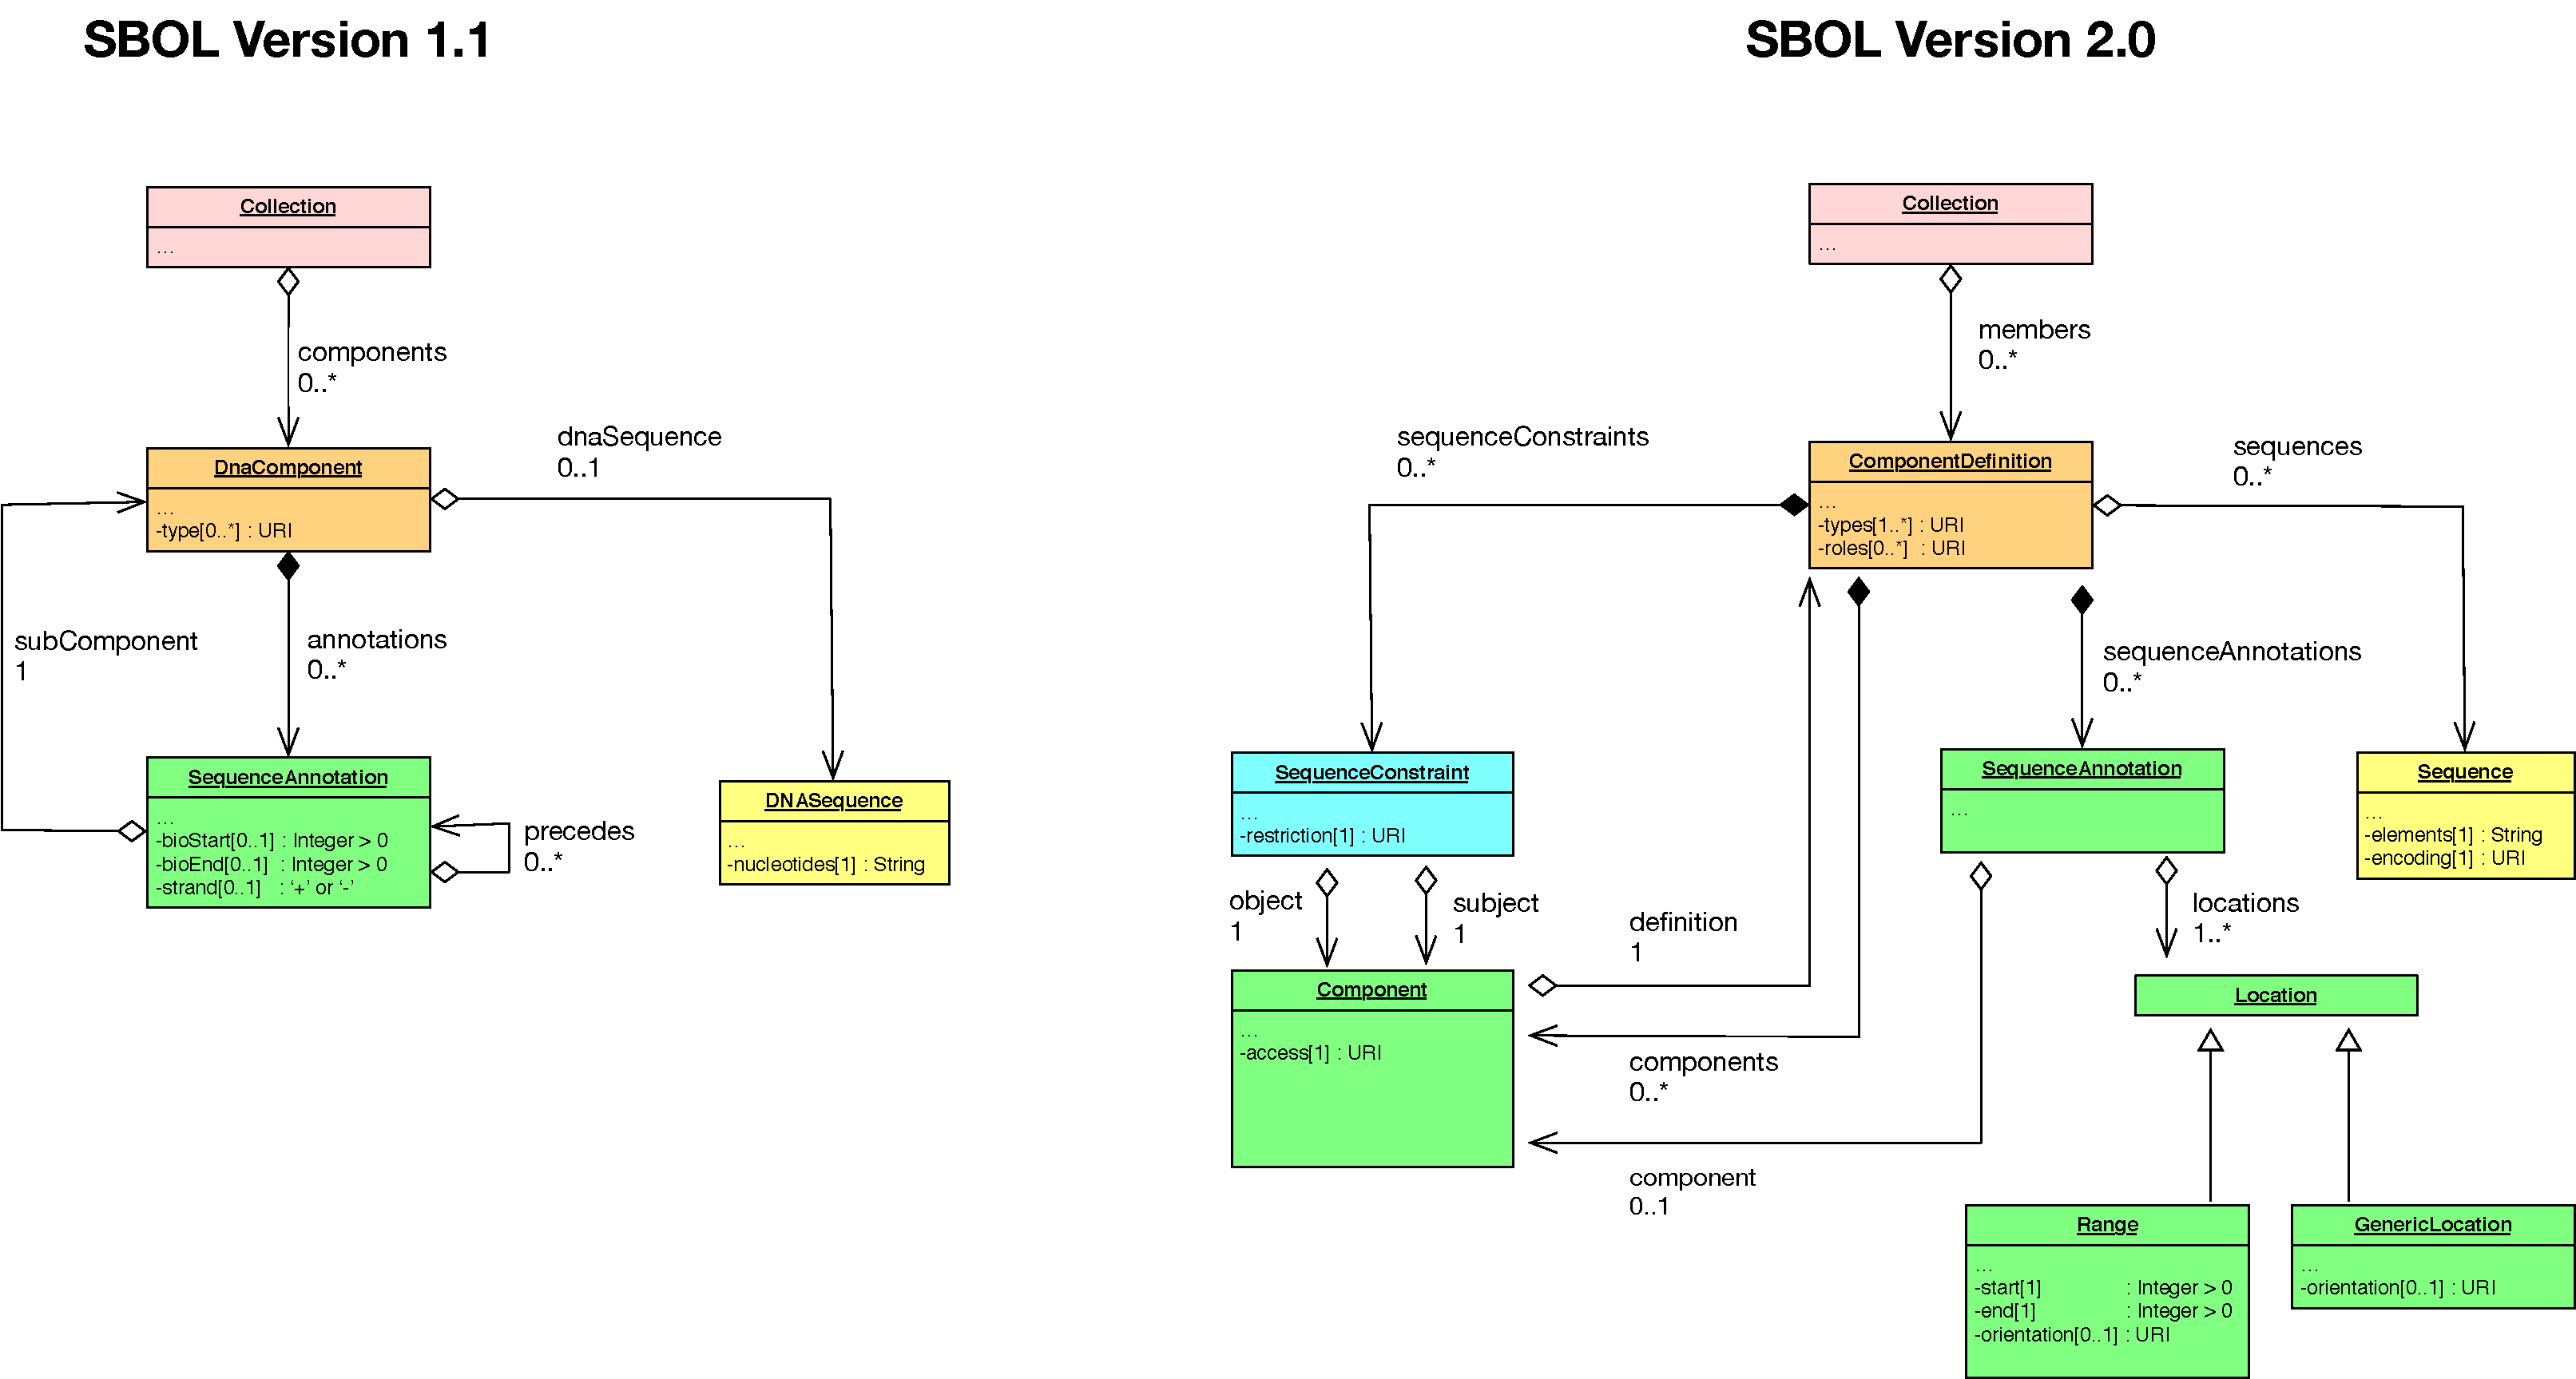
\includegraphics[width=\textwidth]{images/sbol_v1_to_v2}
\end{center}
\caption{\label{SBOL1TO2}The mapping from the SBOL 1.1 data model to the SBOL 2.x  data model, indicating corresponding classes/properties by color.}
\end{figure*}
